%\chapter{Referencial Teórico}\label{cap:background}
\chapter{Literature Revision}\label{cap:background}

\section{Related Work}

%Após uma revisão sistemática da literatura, foram identificadas inúmeras abordagens para a análise de risco: Modelo de Regressão Logística (MRL), Rede de Crenças Bayesiana (RCB), Redes Neurais Artificiais (RNAs), Análise de Discriminantes (AD), Árvore de Decisão (ADE), Algoritmos Genéticos (AG), Otimização por Enxame de Partículas (PSO), Teoria dos Conjuntos Fuzzy (TCF), Sistemas Neuro-Fuzzy (SNF), Mapas Cognitivos Fuzzy Estendidos (E-FCM) \cite{mizuno2001prediction} \cite{huang2004neuro} \cite{hu2007software} \cite{attarzadeh2010novel} \cite{dzega2010classification} \cite{yu2011software} \cite{saxena2012software} \cite{dan2013improving}.
After a systematic literature revision, numerous approaches were explored in risk analysis, that includes Logistic Regression Model (LRM), Bayesian Belief Network (BBN), Artificial Neural Network (ANN), Discriminant Analysis (DA), Decision Tree (DT), Genetic Algorithm (GA), Particle Swarm Optimization (PSO), Fuzzy Set Theory (FST), Neuro-Fuzzy System (NFS), Extended Fuzzy Cognitive Maps (E-FCM) \cite{mizuno2001prediction} \cite{huang2004neuro} \cite{hu2007software} \cite{attarzadeh2010novel} \cite{dzega2010classification} \cite{yu2011software} \cite{saxena2012software} \cite{dan2013improving}.

%Hu et al. \cite{hu2007software} propuseram um método para análise de riscos de software e previsão do resultado de projetos de software. Algoritmos Genéticos foram utilizados como método de otimização do desempenho de Redes Neurais por meio da seleção dos pesos, da estrutura da rede e da regra de aprendizado. A RNA padrão, nesse estudo, teve uma melhoria no desempenho após a inclusão de AG. Os resultados dos experimentos mostraram que após a introdução de AG para o processo de treinamento da RNA, o modelo de avaliação de risco de software modificado pôde ser sensivelmente melhorado alcançando uma maior precisão quando comparado com o modelo SVM. Zhang Dan \cite{dan2013improving} propôs um modelo de previsão baseado em RNA que utiliza o Modelo de Custo Construtivo (COCOMO) que foi aprimorado após a aplicação do PSO, para prover um método de estimativa do esforço no desenvolvimento de software de forma precisa. Attarzadeh e Ow \cite{attarzadeh2010novel} utilizaram a RNA para melhorar a precisão da estimativa do esforço comparado com o modelo tradicional COCOMO. Huang et al. \cite{huang2004neuro} apresentaram um \textit{framework} genérico para a estimativa de software baseado em SNF e melhoraram a estimativa de custo para o COCOMO'81.
Hu et al. \cite{hu2007software} proposed a method to analyze software risks and predict outcomes of software projects. Genetic algorithm could be utilized as an optimization method to improve ANN in many ways, including weights, network structure and rule learning. The standard ANN was enhanced by introducing GA, in that study. Results of the experiments showed that after introducing GA to the ANN training process, the enhanced software risk evaluation model could be improved notably and achieved higher accuracy when compared to the SVM model. Zhang Dan \cite{dan2013improving} proposed an ANN prediction model that incorporates with Constructive Cost Model (COCOMO) which was improved by applying PSO, to provide a method which can estimate the software develop effort accurately. Attarzadeh e Ow \cite{attarzadeh2010novel} utilized ANN to improve accuracy of effort estimation compared to the traditional COCOMO model. Huang et al. \cite{huang2004neuro} have presented a general framework for software estimation based on NFS, the authors improved cost estimation for COCOMO'81.

%Yu \cite{yu2011software} apresentou um modelo baseado na Teoria Fuzzy. Ele superou a dificuldade da avaliação de indicadores qualitativos e quantitativos nos métodos de análise tradicionais. Além disso, Saxena e Singh \cite{saxena2012software} exploraram técnicas Neuro-Fuzzy no projeto de um modelo adequado na utilização de uma melhor estimativa de esforço no desenvolvimento de software para projetos da NASA. Os resultados mostraram que o SNF tem o menor erro de previsão quando comparado com modelos existentes. Por outro lado, Lazzerini e Mkrtchyan \cite{lazzerini2011analyzing} sugeriram um \textit{framework} para análise de riscos usando E-FCM e E-FCM Estendidos, pela introdução de uma representação gráfica especial para análise de risco.
Yu \cite{yu2011software} showed up a model based on the fuzzy theory. He overcame the difficulty of qualitative indicators and quantitative assessment in the traditional analysis methods. In addition, Saxena and Singh \cite{saxena2012software} explored neuro-fuzzy techniques to design a suitable model to utilize improved estimation of software effort for NASA software projects. Results showed that NFS has the lowest prediction error compared with existing models. Meanwhile, Lazzerini and Mkrtchyan \cite{lazzerini2011analyzing} suggested a framework to analyze risks using E-FCMs and extended E-FCMs themselves by introducing a special graphical representation for risk analysis.

%Mizuno et al. \cite{mizuno2001prediction} propuseram um novo método de previsão para projetos de software arriscados. Os autores utilizaram o modelo de regressão logística para estimar se um projeto pode tornar-se arriscado ou não. No entanto, a abordagem de previsão proposta para o custo e a duração não tem um nível alto de precisão. 
Mizuno et al. \cite{mizuno2001prediction} have proposed a new prediction method for risky software projects. The authors have used the logistic regression model to predict whether a project becomes risky or not. However, the proposed estimating approaches for the cost and the duration do not have absolutely high level of accuracy.

%Dzega e Pietruszkiewicz \cite{dzega2010classification} apresentaram resultados de experimentos de análise de riscos realizados usando classificadores de mineração de dados tais como C4.5, RandomTree e Árvore de Regressão e Classificação (CART). Além disso, eles descreveram como os metaclassificadores \textit{boosting} e \textit{bagging} foram aplicados para melhoria dos resultados e também analisaram a influência de seus parâmetros em habilidades de generalização para a precisão da estimativa. Devido a um grande número de atributos desordenados na base de dados, MLP e SVM foram rejeitados prematuramente, gerando baixa precisão para cada conjunto de dados.
Dzega and Pietruszkiewicz \cite{dzega2010classification} have presented results of risk analysis experiments performed using data mining classifiers such as C4.5, RandomTree and Classification and Regression Tree (CART) algorithms. Besides that, they described how boosting and bagging metaclassifiers were applied to improve the results and also analyzed influence of their parameters on generalization abilities in prediction accuracy. Due to a large number of unordered labeled attributes in datasets, MLP and SVM were rejected at early stages, producing low accuracy for each dataset.

%Em resumo, alguns desses estudos propuseram métodos para a estimativa de custo, cronograma e esforço de projetos de software; outros estudos propuseram abordagens para classificação de risco e de projetos de software (sucesso, desafiado ou falho); os demais apresentaram técnicas para estimativa do impacto do risco na gestão de projetos de software \cite{yu2011software} \cite{saxena2012software} \cite{lazzerini2011analyzing} \cite{dzega2010classification}. 
In summary, some of those studies proposed methods to software project cost, schedule and effort estimation; another studies proposed approaches to risk classification and software project classification (success, challenged and failed). Moreover, the remainder presented techniques to risk impact estimation on software project management \cite{yu2011software} \cite{saxena2012software} \cite{lazzerini2011analyzing} \cite{dzega2010classification}.

\section{Project Risk Management}

%Risco pode ser definido como um evento incerto ou condição que, se ocorrer, afeta pelo menos um dos objetivos do projeto. Ele pode ser considerado tanto como uma ameaça (impacto negativo) quanto uma oportunidade (impacto positivo) \cite{PMBOK2008}. 
According to the PMBOK \cite{PMBOK2008}, risk can be defined as an uncertain event or condition that, if it occurs has an effect on at least one of the project goals. It can be considered both a threat (negative impact) or opportunity (positive impact).

%O Gerenciamento de Riscos envolve processos de planejamento, identificação, avaliação e priorização dos mesmos. Numa definição mais apropriada, gerenciamento de riscos pode ser definido como o processo de análise do grau de exposição ao risco e na determinação de como melhor lidar com essa exposição. Essa área objetiva não somente a identificação, como também o desenvolvimento de uma abordagem robusta para gerenciar proativamente o impacto dos riscos no projeto \cite{OSUNDAHUNSI2012}.
Risk management involves planning, identification, assessment and prioritization . In a better definition, risk management can be defined as the process of analyzing the risk exposure and determining how best deal with such exposure. One goal of this area is not only to identify, but also develop a robust approach to proactively manage the impact on the project \cite{OSUNDAHUNSI2012}.

%De acordo com o PMBOK \cite{PMBOK2008}, o gerenciamento de riscos em projetos envolvem processos relativos ao planejamento, identificação, análise, planejamento de respostas, monitoramento e controle de riscos de um projeto. Seu objetivo é aumentar a probabilidade e o impacto dos eventos positivos e reduzir a probabilidade e severidade dos eventos negativos. Do ponto de vista de gerenciamento, a tomada de decisões conscientes pela avaliação do que pode dar errado, assim como a probabilidade e a gravidade do impacto, é o cerne do gerenciamento de riscos. Essa atividade envolve a avaliação das vantagens e desvantagens associadas a todas as alternativas propostas para mitigação de riscos em termos de seus custos, benefícios, riscos e da avaliação do impacto das decisões atuais sobre as alternativas futuras.
According to PMBOK \cite{PMBOK2008}, Project Risk Management includes process as planning, identification, analysis, response planning, monitoring and controlling risks of a project. Its purpose is to increase likelihood and impact of positive events and reduce probability and severity of negative events. From management point of view, making informed decisions by consciously assessing what can go wrong, as well as its likelihood and severity of the impact, is at the heart of risk management. This activity involves the evaluation of the trade-offs associated with all policy options for risk mitigation in terms of their costs, benefits, risks and the evaluation of the impact of current decisions on future options.

%Um resumo dos processos no gerenciamento de riscos é definido a seguir. Seis são os tópicos incluídos nos grupos de atividades de planejamento, monitoramento e controle.
%\begin{itemize}
%\item Planejar o gerenciamento dos riscos: o processo de definição da condução das atividades de gerenciamento de risco num projeto;
%\item Identificar riscos: o processo de determinação dos riscos que possam afetar o projeto e a documentação de suas características;
%\item Realizar a análise qualitativa dos riscos: o processo de priorização dos riscos para análise ou ações adicionais através da avaliação e combinação de suas probabilidades de ocorrência e impacto;
%\item Realizar a análise quantitativa dos riscos: o processo de análise numérica do efeito de riscos identificados previamente, em termos dos objetivos gerais do projeto;
%\item Planejar respostas aos riscos: o processo de desenvolvimento de opções e ações para aumento das oportunidades e diminuição das ameaças aos objetivos do projeto;
%\item Monitorar e controlar os riscos: o processo de implementação do planejamento de respostas aos riscos, rastreamento de riscos identificados, monitoramento dos riscos residuais, identificação de novos riscos e avaliação da eficácia do processo de tratamento de risco durante todo o projeto.
%\end{itemize}
A summary of project risk management processes are defined as follows. There are six topics for project risk management included in the planning and the monitoring and controlling groups.
\begin{itemize}
\item Planning risk management: the process of defining how conduct risk management activities in a project;
\item Identifying risks: the process of determining risks that can affect project and documenting its characteristics;
\item Performing qualitative risk analysis: the process of prioritizing risks to analyze or additional actions through assessment and combination of its occurrence probability and impact;
\item Performing quantitative risk analysis: the process of analyzing numerically the effect of previous identified risks, in terms of general project objectives;
\item Planning risk responses: the process of developing options and actions to increase opportunities and decrease threats to project objetives;
\item Monitoring and controlling risks: the process of implementing risk responses planning, tracking identified risks, monitoring residual risks, identifying new risks and assessing the efficacy of risk treatment process during the whole project.
\end{itemize}

%O \textit{Software Engineering Institute}(SEI) desenvolveu uma metodologia de gerenciamento de risco chamada \textit{Software Risk Evaluation}(SRE) que é especificamente voltada para projetos na indústria de software. O paradigma SRE é composto por seis elementos: cinco módulos (identificação, análise, planejamento, acompanhamento e controle) e um elemento central (comunicação), que é a chave para a efetiva gestão de riscos \cite{HIGUERAHAIMES1996} \cite{williams1999software}.
The Software Engineering Institute (SEI) has developed a risk management methodology named Software Risk Evaluation (SRE) that is specifically oriented to projects in the software industry. The SRE paradigm consists of six elements: five modules (identify, analyze, plan, track, control) and a central element (communication), which is the key to effective risk management \cite{HIGUERAHAIMES1996} \cite{williams1999software}.

%Boehm \cite{BOEHM1991}, Chapman \cite{chapman1996project}, Fairley \cite{fairley1994risk}, Bandyopadhyay et al. \cite{bandyopadhyay1999framework} apresentaram métodos e modelos diferentes de gerenciamento de riscos em projetos de software. No entanto, há elementos em comum em todas as abordagens anteriores: a identificação, a avaliação da probabilidade e impacto, e o planejamento a respostas para manuseio desses riscos se eles ocorrerem \cite{holzmann2011developing}.
Boehm \cite{BOEHM1991}, Chapman \cite{chapman1996project}, Fairley \cite{fairley1994risk}, Bandyopadhyay et al. \cite{bandyopadhyay1999framework} have presented different methods and models for risk management of software projects. However, there are common elements in all previous approaches: identification, assessment of the likelihood and impact, and responses planning to manage these risks if they occur.

%O gerenciamento de risco, no sentido amplo, é útil para organizações que têm um portfólio de projetos. Esse gerenciamento foca principalmente no risco agregado para a tomada de decisões como interromper, abortar e continuar com a realização do projeto. No entanto, na perspectiva de um líder de projetos, há apenas projetos isolados, em que o enfoque está centrado em cada uma das atividades para cada projeto. Segundo Kendrick \cite{kendrick2003identifying}, o gerenciamento de risco de projetos deve focar em riscos no sentido restrito.
Risk management in the large sense is useful to organizations, where many projects are undertaken. That management has main focus on aggregate risk for decision making such as interrupt, abort and continuing. Otherwise, in project leader perspective, there are only isolated projects, that should focus primarily on risk in the small sense \cite{kendrick2003identifying}.

%Já no sentido restrito, serve para melhorar as chances de cada projeto individual alcançar o sucesso. Na maioria dos outros campos, o gerenciamento de risco está preocupado principalmente com os valores médios de um grande número de eventos independentes. Para o gerenciamento do risco de projetos, no entanto, o que geralmente mais importa é a previsibilidade - gerenciar a variação esperada	no resultado para o projeto específico \cite{kendrick2003identifying}.
Otherwise in the small sense, works to improve the chances for each individual project. In most other fields, risk management is primarily concerned with the mean values of large numbers of independent events. For project risk management, however, what generally matters most is predictability - managing the variation expected in the result for the specific project \cite{kendrick2003identifying}.

%Os objetivos da gestão de risco para um único projeto são estabelecer um plano crível, consistente com os objetivos de negócio, e na minimização do intervalo de resultados possíveis. Quanto maior o intervalo de duração possível para um projeto mais elevado o seu risco. O risco do projeto aumenta com o nível de incerteza, tanto negativa quanto positiva \cite{kendrick2003identifying}.
The goals of risk management for a single project are to establish a credible plan consistent with business objectives and then to minimize the range of possible outcomes. The larger range of possible durations for a project represents higher risk. Project risk increases with the level of uncertainty, both negative and positive \cite{kendrick2003identifying}.

%O gerenciamento do risco de projetos utiliza dois parâmetros fundamentais de risco: probabilidade e perda. Probabilidade é geralmente a possibilidade de um evento ocorrer - como é frequentemente obtida através de suposição, logo pode ser bastante imprecisa. Perda é geralmente designado em projetos como "impacto", e baseia-se nas consequências para o projeto no caso de ocorrência do risco. Impacto é geralmente medido em tempo ou custo, particularmente para avaliação quantitativa de riscos \cite{kendrick2003identifying}.
Project risk management uses the two fundamental parameters of risk - likelihood and loss. Likelihood is generally the probability of a project event occur - though often by guessing, so it can be quite imprecise. Loss is generally referred to for projects as "impact", and it is based on the consequences to the project if the risk does occur. Impact is usually measured in time or cost, particularly for quantitative risk assessment \cite{kendrick2003identifying}.

%O principal benefício do gerenciamento de riscos em projetos é tanto o desenvolvimento de uma base de credibilidade para cada projeto, mostrando que o mesmo é possível, quanto da demonstração da inviabilidade do projeto, mostrando que o mesmo deva ser evitado, abortado ou transformado. A análise de risco pode também revelar oportunidades para melhoria dos projetos que podem resultar em altos retornos no investimento. Quando realizada de forma adequada reduz tanto o custo total quanto a frustração causada por problemas evitáveis. A quantidade de retrabalho e atraso imprevisto de esforço no projeto é reduzida. Além disso, ela revela fraquezas num plano de projeto e desencadeia mudanças, novas atividades e realocação de recursos que melhoram o resultado do projeto \cite{kendrick2003identifying}.
The primary benefit of project risk management is either to develop a credible foundation for each project by showing that it is possible, or to demonstrate that the project is not feasible so it can be avoided, aborted, or transformed. Risk analysis can also reveal opportunities for improving projects that can result in increased project value. Adequate risk analysis lowers both the overall cost and the frustration caused by avoidable problems. The amount of rework and unforeseen late project effort is reduced. Besides that, risk analysis uncovers weakness in a project plan and triggers changes, new activities, and resource shifts that improve the project \cite{kendrick2003identifying}.

\subsection{Qualitative Risk Analysis}

%O processo de análise qualitativa avalia as características dos riscos de projetos identificados individualmente e prioriza-os baseado nas requisições estabelecidas para o projeto. Em outras palavras, a análise qualitativa avalia a probabilidade de cada evento ocorrer e o efeito individual de cada um deles nos objetivos do projeto. Como tal processo não aborda diretamente o risco global para os objetivos do projeto, que resultam do efeito combinado dos eventos individuais e as interações entre si, então isso pode ser obtido através do uso de técnicas de análise quantitativa \cite{PRACTICESTANDARD2009}.
The process of qualitative analysis evaluates the characteristics of project risks identified individually and prioritizes them based on requirements established for the project. In other words, qualitative analysis assesses the probability of each event occurring and the individual effect of each of them to the project objectives. As that process does not directly address the overall risk to the project objectives, which result from the combined effect of individual events and their interactions with each other, then this can be achieved through the use of techniques of quantitative analysis \cite{PRACTICESTANDARD2009}.

\subsection{Quantitative Risk Analysis}

%Análise é a conversão de dados de risco em informação para tomada de decisão. A análise fornece a base para o gerente de projetos trabalhar nos riscos certos e mais críticos. Boehm \cite{BOEHM1991} define o objetivo da análise de risco como a avaliação da probabilidade e magnitude de perda para cada item de risco identificado, e ele avalia os riscos compostos das interações dos itens de risco. Técnicas típicas incluem modelos de desempenho e custo, análise de rede, análise de decisão estatística e análise de fatores de qualidade (tais como confiabilidade, disponibilidade e segurança).
Analysis is the conversion of risk data into risk decision-making information. Analysis provides the basis for the project manager to work on the "right" and most critical risks. Boehm \cite{BOEHM1991} defines risk analysis objective as the assessment of the loss probability and loss magnitude for each identified risk item, and it assess compound risks in risk-item interactions. Typical techniques include performance and cost models, network analysis, statistical decision analysis and quality-factor (such as reliability, availability, and security) analysis.

%A análise de risco depende de um bom mecanismo de identificação de riscos. No entanto, a maioria dos métodos assume que os gerentes devam ter a experiência necessária a respeito de todos os fatores de risco pertinentes, o que nem sempre corresponde a realidade. Além disso, muitos desses métodos podem ser demorados e, portanto, muito dispendiosos para se utilizar de forma regular. Portanto, um método popular para a identificação de fatores de risco tem sido a utilização de listas de verificação. Infelizmente, essas listas de verificação são baseadas em pequenas amostras ou, ainda pior, viciadas pelos seus métodos de coleta de dados históricos de risco.
Risk analysis depends on a good mechanism to identify risks. However, most of the methods assume that managers have the required experience to be aware of all pertinent risk factors, but it can not be the situation. Moreover, many of these methods can be time-consuming and thus too costly to use on a regular basis. Therefore, one popular method for identifying risk factors has been the use of checklists. Unfortunately, these checklists are based in small samples or, even worse, flawed in their risk historical data collection methods.

%As técnicas mais utilizadas para análise de risco incluem \cite{PMBOK2008}:
%\begin{itemize}
%\item Análise de Sensibilidade: ajuda a determinar quais riscos têm os maiores impactos potenciais no projeto. Uma representação típica disso é o diagrama de tornado (explicar isso);
%\item Valor Monetário Agregado(EMV): é um conceito estatístico que calcula o valor médio do impacto do risco agregado quando o futuro inclui cenários que podem ou não ocorrer (ou seja, sob a análise da incerteza). Um uso comum desse tipo de técnica é a análise da árvore de decisão;
%\item Modelagem e simulação: simulação utiliza um modelo que converte as incertezas especificadas e detalhadas em seu potencial impacto sobre os objetivos do projeto. As simulações iterativas gerais são realizadas usando Simulação de Monte Carlo;
%\item Opinião especializada: opinião especializada (de especialistas com experiência relevante e recente) é necessária não apenas para identificação dos impactos potenciais sobre o custo e o cronograma e para avaliação da probabilidade, como também para definir as variáveis de entrada e quais ferramentas utilizar.
%\end{itemize}
Most used techniques to risk analysis include \cite{PMBOK2008}:
\begin{itemize}
\item Sensibility analysis: it helps to determine which risks have the higher potential impact on the project. A typical representation of the sensitivity analysis is the tornado diagram;
\item Earned Monetary Value (EMV): it is a statistical concept that computes the average score when the future includes scenarios that may or may not occur (ie, under uncertainty analysis). A common use of this kind of technique is the decision tree analysis;
\item Modeling and simulation: Simulation utilizes a model that converts the detailed specified uncertainties in their potential impact on project objectives. The general iterative simulations are performed using MCS;
\item Specialized opinion: expert judgment (ideally by specialists with relevant and recent expertise) is required to identify the potential impacts on cost and schedule, to assess the likelihood, but also to define input variables and which tools to use.
\end{itemize}

%O objetivo da análise quantitativa de riscos é criar um "perfil do risco" do projeto. Para tanto, são necessárias as seguintes informações: a chance de o projeto ser finalizado dentro de um certo período de tempo ou orçamento; a taxa de sucesso de projetos; as estimativas de pior caso, médio e melhor caso e outros parâmetros do projeto \cite{PMBOK2008}.
The purpose of a quantitative risk analysis is to create a "risk profile" of the project. For this purpose the following information are required: the chance of finishing the project within a certain period of time or budget; the success rate of projects; the worst, average and best estimates of duration and other project parameters \cite{PMBOK2008}.

%Alguns trabalhos propõem novas ferramentas de análise quantitativa de riscos. Entre eles, Virine \cite{VIRINE2009} apresenta a metodologia da Cadeia de Eventos. Nesse trabalho, as atividades de um projeto não são um procedimento uniforme e contínuo. Essas tarefas são afetadas por eventos externos, que transformam as atividades de um evento para outro. O momento em que os eventos externos ocorrem são probabilísticos e podem ser definidos utilizando uma distribuição estatística. Além disso, eventos podem causar outros eventos, criando, portanto, a Cadeia de Eventos. A análise dessas combinações é realizada através da Simulação de Monte Carlo.
Some studies propose new tools for quantitative risk assessment. Among them, Virine \cite{VIRINE2009} presents the methodology Events Chain. In that paper, the activities of a project are not an uniform and continuous process, those tasks are affected by external events, that transform the activities from one event to another. The moment at which external events occur are probabilistic and can be set using a statistical distribution. Moreover, events can cause other events, thereby, creating the Event Chain. The analysis of those combinations is performed by Monte Carlo simulation.

%A análise de risco demonstra a incerteza dos resultados do projeto e é útil para justificar reservas de cronograma e/ou recursos. É mais apropriado para definir uma janela de tempo (ou orçamento) em vez de um objetivo único para projetos arriscados. Por exemplo, o cronograma alvo para um projeto arriscado pode ser doze meses, mas o cronograma empenhado, refletindo problemas potenciais, pode ser fixado em quatorze meses. A conclusão no prazo (ou antes) desse intervalo define um projeto de sucesso; somente se o projeto demorar mais de quatorze meses será considerado um fracasso \cite{kendrick2003identifying}.
Risk analysis demonstrates the uncertainty of project outcomes and is useful in justifying reserves for schedule and/or resources. It is more appropriate to define a window of time (or budget) instead of a single-point objective for risky projects. For example, the target schedule for a risky project might be twelve months, but the committed schedule, reflecting potential problems, may be set at fourteen months. Completion within (or before) this range defines a successful project; only if the project takes more than fourteen months will it be considered a failure \cite{kendrick2003identifying}.

\section{Conventional Techniques for Risk Analysis}

\subsection{Monte Carlo Simulation}

%A Simulação de Monte Carlo é uma técnica que computa ou itera o custo ou cronograma do projeto muitas vezes usando valores de entrada selecionados aleatoriamente a partir de distribuições de probabilidades de custos ou durações possíveis, para calcular uma distribuição dos custos totais ou datas de finalização do projeto \cite{PMBOK2008}.
Monte Carlo simulation is a technique that computes or iterates the project cost or schedule many times using input values selected at random from probability distributions of possible costs or durations, to calculate a distribution of possible total project cost or completion dates \cite{PMBOK2008}.

%Um modelo é desenvolvido, e ele contém algumas variáveis de entrada. Essas variáveis de entrada tem resultados possíveis diferentes, representados por uma função de distribuição de probabilidade de valores para cada variável. O método de Monte Carlo é uma abordagem de simulação através de computação intensiva para determinar a probabilidade de resultados possíveis de um objetivo do projeto, tais como a data de finalização ou o custo total. As entradas do procedimento são obtidas aleatoriamente a partir de intervalos específicos com funções de distribuição de probabilidade para as durações das atividades no cronograma ou itens da linha de base de custo. Esses diferentes valores de entrada são utilizados não apenas para construir um histograma de resultados possíveis para o projeto e sua probabilidade relativa, mas também a probabilidade cumulativa para calcular as reservas de contingências desejadas para o cronograma ou custo. Resultados adicionais incluem a importância relativa de cada entrada para determinar o custo e o cronograma geral para o projeto \cite{kwak2007exploring}.
A model is developed, and it contains certain input variables. These variables have different possible values, represented by a probability distribution function of the values for each variable. The Monte Carlo method is a detailed simulation approach through intensive computing to determine the likelihood of possible outcomes of a project goal; for example, the completion date or total cost. The inputs of the procedure are obtained randomly from specific intervals with probability distribution functions for the durations of schedule activities or items from cost baseline. Those different input values are used to construct a histogram of possible results to the project and its relative probability, but also the cumulative probability to calculate desired contingency reserves for time or cost. Additional results include the relative importance of each input in determining the overall project cost and schedule \cite{kwak2007exploring}.

%O desenvolvimento desse método, especialmente o uso de computadores para realizar os cálculos, foi creditado a Stanislaw Ulam, um matemático que trabalhou no Projeto Americano de Manhattan durante a Segunda Guerra Mundial. O seu trabalho com Jon von Neuman e Nicholas Metropolis transformaram a amostragem estatística de uma curiosidade matemática para uma metodologia formal aplicável a uma grande variedade de problemas \cite{kwak2007exploring}. 
The invention of the method, especially the use of computers to do the calculations, was credited to Stanislaw Ulam, a mathematician working in the U.S. Manhattan Project during World War II. His work with Jon von Neumann and Nicholas Metropolis turned statistical sampling from a mathematical curiosity to a formal methodology applicable to a wide range of problems \cite{kwak2007exploring}.

%A Simulação de Monte Carlo é uma abordagem detalhada de simulação através de computação intensiva para determinar a probabilidade de resultados possíveis de um objetivo do projeto; por exemplo, a data de conclusão ou o custo total. As entradas para o procedimento são obtidas aleatoriamente a partir de intervalos específicos com funções de distribuição de probabilidade para as durações das atividades do cronograma ou itens da linha de custo. Esses valores de entrada diferentes são usados para construir um histograma de possíveis resultados do projeto e sua probabilidade relativa, como também, a probabilidade cumulativa para calcular as reservas de contingência desejadas de tempo ou custo. Resultados adicionais incluem a importância relativa de cada entrada na determinação do custo geral do projeto e cronograma. Um exemplo de resultados de estimativa de riscos de cronograma e custo são apresentados na Figura \ref{fig:montecarlo} \cite{PRACTICESTANDARD2009}.
Monte Carlo Simulation is a detailed simulation approach through intensive computation to determine the likelihood of possible outcomes of a project objective, for example, the completion date or the overall cost. The inputs to the procedure are obtained randomly from specific intervals with probability distribution functions for durations of schedule activities or items in costs baseline. Such distinct input values are used to construct a histogram of possible outcomes and relative probability in project, as well as the cumulative probability to calculate the desired contingency reserve of time or cost. Additional results include the relative importance of each input to determine the overall project cost or the project schedule. An example of prediction of schedule and cost risks are presented in Figure \ref{fig:montecarlo} \cite{PRACTICESTANDARD2009}.

%Na Figura \ref{fig:montecarlo}, observa-se a previsão de finalização para um cronograma de um projeto. No eixo horizontal, encontram-se as possíveis datas de finalização do cronograma, a frequência de ocorrência dessas datas na amostragem são representadas pelas barras verticais, a frequência cumulativa é representada pela curva escura e pelos respectivos valores na borda direita do gráfico. A partir da frequência relativa, é possível prever a probabilidade do projeto finalizar até determinada data, nesse exemplo, esse projeto teve 90\% de chance de finalizar até 08 de Maio de 2009.
In Figure \ref{fig:montecarlo}, it is observed the forecast of a timeline for completion of a project. On the horizontal axis, there are the possible end dates of the timeline. How often those dates occur in sampling are represented by vertical bars. The cumulative frequency is represented by the dark curve and each related value is on the right edge of the chart. Based on the relative frequency, it is possible to predict the likelihood of the project be completed by a given date, int that example, the illustrated project has a 90\% chance to finish until May 8, 2009.

\begin{figure}[h]
	\centering
	\includegraphics[width=.6\textwidth]{image/montecarlo.png}
	\caption{Exemplo de Resultado da Simulação Monte Carlo}
	\label{fig:montecarlo}
	%Traduzir para o Português.
\end{figure}

\subsection{PERT Analysis}

%PERT foi criada pela Marinha dos EUA em 1958 como uma ferramenta para programar o desenvolvimento de um sistema de armamento por completo. A técnica considera o projeto sendo uma rede acíclica de eventos e atividades. A duração de um projeto é determinada por um plano de fluxo do sistema no qual a duração de cada atividade tem um valor esperado e uma variância. O caminho crítico inclui uma sequência de atividades que não podem ser adiadas, sem ameaçar o projeto por inteiro. PERT pode ser usado para estimar a probabilidade de completar um projeto ou atividades individuais por qualquer período de tempo especificado. É também possível determinar a duração do intervalo de tempo correspondente a uma dada probabilidade \cite{cottrell1999simplified}.
PERT was originated by the U.S. Navy in 1958 as a tool for scheduling the development of a complete weapons system. The technique considers a project to be an acyclic network of events and activities. The duration of a project is determined by a system flow plan in which the duration of each task has an expected value and a variance. The critical path includes a sequence of activities that cannot be delayed without jeopardy to the entire project. PERT can be used to estimate the probability of completing either a project or individual activities by any specified time. It is also possible to determine the time duration corresponding to a given probability \cite{cottrell1999simplified}.

%O primeiro passo na aplicação do PERT é desenvolver diagramas da rede do projeto, em que cada arco representa uma atividade e cada nó simboliza um evento (como o início ou conclusão de uma tarefa). Alternativamente, cada nó pode simbolizar uma atividade. O segundo passo é designar três estimativas de tempo para cada tarefa: otimista $(a)$, pessimista $(b)$ e mais provável $(m)$. Pequenas probabilidades estão associadas com $a$ e $b$.No diagrama original, $a$ é a duração mínima de uma atividade; a probabilidade de uma duração mais curta é zero. Da mesma forma,  $b$ é a duração máxima; a probabilidade de uma duração menor ou igual a $b$ é 100\%. Nenhuma suposição é feita sobre a posição de $m$ relativo a $a$ e $b$. Em termos estatísticos,  $a$ e $b$ são os extremos de uma distribuição hipotética de tempos de duração. A moda da distribuição é $m$. Para acomodar a flexibilidade nas posições destes parâmetros, a distribuição beta é usada. A distribuição beta é útil para a descrição de dados empíricos e pode ser simétrica ou enviesada \cite{cottrell1999simplified}.
The first step in applying PERT is to diagram the project network, in which each arc represents an activity and each node symbolizes an event (such as the beginning or completion of a task). Alternatively, each node can symbolize an activity. The second step is to designate three time estimates for each task: optimistic $(a)$, pessimistic $(b)$ and most likely $(m)$. Small probabilities are associated with $a$ and $b$. In the original PERT, $a$ is the minimum duration of an activity; the probability of a shorter duration is zero. Similarly, $b$ is the maximum duration; the probability that the duration will be less than or equal to $b$ is 100\%. No assumption is made about the position of $m$ relative to $a$ and $b$. In statistical terms, $a$ and $b$ are the extreme ends of a hypothetical distribution of duration times. The mode of the distribution is $m$. To accommodate flexibility in the positions of these parameters, the beta distribution is used. The beta distribution is useful for describing empirical data and can be either symmetric or skew \cite{cottrell1999simplified}.

%O terceiro passo é calcular o valor esperado e variância da duração de cada atividade no diagrama de rede do projeto. A média de uma distribuição beta é uma equação cúbica. A equação para essa média, Equação \ref{eq:mediaPERT}, é uma aproximação linear dessa forma:
The third step is to compute the expected value and variance of the duration of each activity in the project network. The mean of a beta distribution is a cubic equation. The PERT equation for the mean, Equation \ref{eq:mediaPERT}, is a linear approximation to this:

\begin{equation}
\label{eq:mediaPERT}
\tau_e = (\alpha + 4m + \beta) / 6
\end{equation}

%onde $\tau_e$ é a duração estimada de uma atividade, $m$ é igual à moda, que ocorre quando $a$ e $b$ são simétricos com relação a $m$.
where $\tau_e = $ is the expected duration of an activity, $m$ is equal to the mode, which occurs when $a$ and $b$ are symmetrical about $m$.

%Em distribuições de probabilidade unimodais, o desvio-padrão da distribuição é igual a cerca de um sexto do intervalo. Com  100\% das durações possíveis vinculadas a $a$ e $b$, a variação estimada da duração é como se segue:
In unimodal probability distributions, the standard deviation of the distribution is equal to approximately one-sixth of the range. With 100\% of the possible durations bound by $a$ and $b$, the estimated variance of the duration is as follows:

\begin{equation}
\label{eq:varianciaPERT}
\sigma^2_100(\tau_e) = [(b - a) / 6]^2
\end{equation}

%onde $\sigma^2$ é a variância da duração da atividade. Uma alternativa, apresentada em \cite{cottrell1999simplified}, é definir $a$ e $b$ como os limiares de 5\% e 95\% do intervalo, respectivamente. Então, a variância é como se segue:
where $\sigma^2$ = variance of the activity duration. An alternative, presented in \cite{cottrell1999simplified} is to define $a$ and $b$ as the 5\% and 95\% thresholds of the range, respectively. Then, the variance is as follows:

\begin{equation}
\label{eq:variancia2PERT}
\sigma^2_90(\tau_e) = [(b - a) / 3.2]^2
\end{equation}

%O quarto passo é ordenar as atividades em seqüência, do início ao fim do projeto, em um formato tabular, listando as durações otimista, pessimista, mais prováveis, esperadas e as variâncias. Em quinto lugar, os passos \textit{forward} e \textit{backward} através da rede são realizadas para identificar o caminho crítico, tal como no método do caminho crítico amplamente utilizado. O teorema limite central é então aplicado como se segue: a distribuição da soma das durações previstas das atividades ao longo do caminho crítico é aproximadamente a distribuição normal, particularmente a medida que o número de atividades aumenta. A duração esperada de cada soma é igual à soma das durações esperadas. Do mesmo modo, a variação de cada soma é a soma das variâncias \cite{cottrell1999simplified}.
The fourth step is to order the activities sequentially, from the beginning to the end of the project, in a tabular format, listing the optimistic, pessimistic, most likely, and expected durations and the variances. Fifth, forward and backward passes through the network are performed to identify the critical path, just as in the widely used critical path method. The central limit theorem is then applied as follows: The distribution of the sum of the expected durations of the activities along the critical path is approximately normal, particularly as the number of activities increases. The expected duration of each sum is equal to the sum of the expected durations. Similarly, the variance of each sum is the sum of the variances \cite{cottrell1999simplified}.

%Essas aplicações do teorema do limite central permitir o cálculo de probabilidades de duração do projeto usando os desvios a partir de uma média zero da variável normal $(Z)$. Essas probabilidades podem ser cruciais na tomada de decisões financeiras quanto à viabilidade de um projeto \cite{cottrell1999simplified}.
These applications of the central limit theorem enable the computation of project duration probabilities using the deviations from a zero mean of the standard normal variable $(Z)$. These probabilities can be critical in making financial decisions about the viability of a project. 

\section{Statistical and Intelligent Computing Techniques for Risk Analysis}

%Nesta seção, serão explorados inicialmente dois modelos de previsão que poderiam ser aplicados para o domínio de análise de risco: regressão linear múltipla e modelos de árvore de regressão. A escolha não foi conseqüência de alguma etapa de seleção formal de modelos, contudo, ainda assim, os modelos apresentam-se como duas boas alternativas para problemas de regressão como são bastante diferentes em termos de suas suposições sobre a "forma" da função de regressão sendo aproximada e pela facilidade de interpretar e velocidade para rodar em qualquer computador. O objetivo da escolha desses dois modelos de regressão comuns  está relacionado com a validação do desempenho de outras técnicas. Por exemplo, se uma técnica de previsão tem um desempenho pior do que modelos de regressão múltipla linear, como de árvores de regressão, então parece ser uma alternativa inadequada.
In this section we will initially explore two different predictive models that could be applied to risk analysis domain: multiple linear regression and regression tree models. Our choice was was not a consequence of some formal model selection step, regarding these models. Otherwise, the models still are two good alternatives for regression problems as they are quite different in terms of their assumptions regarding the "shape" of the regression function being approximated and they are easy to interpret and fast to run on any computer.  The purpose of choosing these two common regression models is to validate the performance of others techniques. For example, if a technique has worse perfformance than multiple linear regression either regression tree models then it seems a bad alternative.

\subsection{Multiple Linear Regression}

%A Regressão Linear Múltipla está entre as técnicas de análise de dados estatísticos mais utilizadas. Esse modelo obtém uma função aditiva relacionando uma variável de saída a um conjunto de variáveis de entrada. Essa função aditiva é a soma de elementos da fórmula $\beta_i \times X_i$, onde $X_i$ é uma matriz estimadora de variáveis e $\beta_i$ é a matriz de pesos na regressão linear múltipla \cite{torgo2003data}
Multiple Linear Regression is among the most used statistical data analysis techniques. These models obtain an additive function relating a target variable to a set of predictor variables. This additive function is a sum of elements of the formula $\beta_i \times X_i$, where $X_i$ is a predictor variable matrix and $\beta_i$ is the weight matrix in the multiple linear regression \cite{torgo2003data}.

%Na regressão linear, os dados são modelados para caber numa linha reta. Por exemplo, uma variável aleatória $Y$, chamada variável de resposta, pode ser modelada como uma função linear de uma variável aleatória $X$, chamada de variável de previsão com a Equação \ref{eq:mlr}:
In linear regression, the data are modeled to fit a straight line. For example, a random variable $Y$, called a response variable, can be modeled as a linear function of another random variable $X$, called a predictor variable with the Equation \ref{eq:mlr}:

\begin{equation}
\label{eq:mlr}
Y = \alpha + \beta X,
\end{equation}

%onde a variância de $Y$ é assumida ser constante. Os coeficientes $\alpha$ e $\beta$ (chamados coeficientes de regressão) especificam o interceptação de $Y$ e a inclinação da linha, respectivamente. Esses coeficientes podem ser resolvidos pelo método dos mínimos quadrados, que minimiza o erro entre a linha real separando os dados e a estimativa da linha. Dado $s$ amostras ou pontos de dados da forma  $(x_1,y_1), (x_2,y_2), ..., (x_s,y_s)$, então os coeficientes de regressão podem ser estimados usando esse método por meio das Equações \ref{eq:betamlr} and \ref{eq:alphamlr}:
where the variance of $Y$ is assumed to be constant. The coefficients $\alpha$ and $\beta$ (called regression coefficients) specify the $Y$ intercept and slope of the line, respectively. These coefficients can be solved for by the method of least squares, which minimizes the error between the actual line separating the data and the estimate of the line. Given $s$ samples or data points of the form $(x_1,y_1), (x_2,y_2), ..., (x_s,y_s)$, then the regression coefficients can be estimated using this method with Equations \ref{eq:betamlr} and \ref{eq:alphamlr}:

\begin{equation}
\label{eq:betamlr}
\beta = \frac{\sum\limits_{i=1}^{s} (x_i - x) (y_i - y) }{\sum\limits_{i=1}^{s} (x_i - x)^2},
\end{equation}

\begin{equation}
\label{eq:alphamlr}
\alpha = y - \beta x,
\end{equation}

%onde $x$ é a média de $x_1,x_2,...,x_s$, e $y$ a média de $y_1,y_2,...,y_s$. Os coeficientes $\alpha$ e $\beta$ frequentemente provêm boas aproximações mesmo para equações de regressão complexas. A regressão múltipla é uma extensão da regressão linear, permitindo uma resposta variável $Y$ para ser modelada como uma função linear de um vetor de características multidimensional \cite{han2006data}.
where $x$ is the average of $x_1,x_2,...,x_s$, and $y$ is the average of $y_1,y_2,...,y_s$. The coefficients $\alpha$ and $\beta$ often provide good approximations to otherwise complicated regression equations. Multiple regression is an extension of linear regression allowing a response variable $Y$ to be modeled as a linear function of a multidimensional feature vector \cite{han2006data}.

\subsection{Regression Tree Model}

%Uma árvore de regressão é uma hierarquia de testes lógicos em algumas das variáveis explanatórias do modelo. Logo, nem todas as variáveis aparecem na árvore. Uma árvore é lida do nó-raiz para os nós-folha. Cada nó da árvore tem dois galhos. Eles estão relacionados ao valor de um teste em cada uma das variáveis de previsão. O teste continua até um nó-folha ser alcançado. Nesses nós-folha tem-se os valores previstos pela árvore. Isso significa que se é necessário usar uma árvore para obter-se uma estimativa para uma amostra particular, é necessário seguir um galho do nó-raiz até um nó-folha, de acordo com os resultados do teste para a amostra. O valor médio da variável alvo encontrado no nó-folha alcançado é a previsão da árvore \cite{torgo2003data} \cite{breiman1984classification}. 
A regression tree is a hierarchy of logical tests on some of the explanatory variables; thus, not all variables need to appear in the tree. A tree is read from the root node to leaf nodes. Each node of a tree has two branches. These are related to the outcome of a test on one of the predictor variables. The testing goes on until a leaf node is reached. At these leaves we have the predictions of the tree. This means that if it is necessary to use a tree to obtain a prediction for a particular sample, it is needed to follow a branch from the root node until a leaf, according to the outcome of the tests for the sample. The average target variable value found at the leaf reached is the prediction of the tree \cite{torgo2003data}.

\begin{figure}[h]
  \centering
  \includegraphics[width=\columnwidth]{image/regressiontreemodel.pdf}
  \caption{Regression Tree Model for PERIL}
  \label{fig:rtm}
\end{figure}

%A Figura \ref{fig:rtm} apresenta o modelo de árvore de regressão para a base de dados do PERIL. Partindo do nó-raiz é possível verificar dois galhos que mostram testes lógicos para a variável \textit{Date0}. Os próximos nós representam resultados possíveis levando-se em conta somente \textit{Date0}. O segundo nível da árvore mostra testes lógicos associados às variáveis \textit{Category3} e \textit{Subcat2}. Em seguida, encontram-se três nós-folha. Cada valor do nó-folha representa os possíveis resultados e o número de amostras no PERIL, que satisfazem os testes lógicos conjugados nos níveis anteriores da árvore. Por último, testes lógicos para a variável \textit{Subcat0} são apresentados para geração de outros dois nós-folha.
Figure \ref{fig:rtm} presents the regression tree model to PERIL dataset. From the root node it is possible to verify two branches, these branches shows logical tests under \textit{Date0} variable. The following nodes represents possible outcomes taking into account only \textit{Date0}. The second level shows logical tests under \textit{Category3} and \textit{Subcat2} variables. Next, it is found three leaf nodes. Each leaf node values represents the possible outcome and the number of samples in PERIL dataset, satisfying the conjugated logical tests in the previous tree levels. Lastly, logical tests under \textit{Subcat0} variable is presented to generate two another leaf nodes.

%Árvores são obtidas geralmente em dois passos. Inicialmente, uma grande árvore é desenvolvida, e em seguida essa árvore é podada eliminando os nós inferiores através de um processo de previsão estatística. Esse processo tem o objetivo de evitar o \textit{overfitting}. Isso tem a ver com o fato de que uma árvore larga demais irá memorizar os dados do treinamento quase perfeitamente, mas irá capturar relações espúrias do conjunto de dados oferecido, e portanto irá ter um desempenho ruim quando exposta a uma nova amostra de dados para a qual previsões são necessárias. O problema de \textit{overfitting} ocorre em muitas técnicas de modelagem, particularmente quando as suposições acerca da função a ser aproximada têm menor importância. Esses modelos, mesmo que tenham uma ampla faixa de aplicação (devido a essas condições não prioritárias), sofrem com esse problema de \textit{overfitting}, necessitando, portanto, de uma previsão baseada em estatística para diminuir o impacto desse efeito \cite{torgo2003data}.
Trees are usually obtained in two steps. Initially, a large tree is grown, and then this tree is pruned by deleting bottom nodes through a process of statistical estimation. This process has the goal of avoiding overfitting. This has to do with the fact that an overly large tree will fit the training data almost perfectly, but will be capturing spurious relationships of the given dataset (overfitting it), and thus will perform badly when faced with a new data sample for which predictions are required. The overfitting problem occurs in many modeling techniques, particularly when the assumptions regarding the function to approximate are more relaxed. These models, although having a wider application range (due to these relaxed criteria), suffer from this overfitting problem, thus requiring a posterior, statistically based estimation step to preclude this effect \cite{torgo2003data}.

\section{Artificial Neural Networks}

%Uma Rede Neural Artificial (RNA) é um processador distribuído maciçamente paralelo constituído por unidades de processamento simples, que tem a propensão natural para armazenar conhecimento experimental e torná-lo disponível para o uso \cite{linlee1996neuralfuzzy}. Ela adota estimativas de regressão não-paramétricas constituída de elementos de processamento interconectados entre dados de entrada e saída, e tem uma excelente capacidade de aprendizado e generalização.
An Artificial Neural Network (ANN) is a massively parallel distributed processor made up of simple processing units, which has a natural propensity to load experimental knowledge and become it available for use  \cite{linlee1996neuralfuzzy}. It adopts non-parametric regression estimates made up of a number of interconnected processing elements between input and output data. They have excellent learning and generalizing capabilities.

%Outra definição descreve uma RNA como um sistema constituído de elementos de processamento, chamados neurônios, os quais estão dispostos em camadas (uma camada de entrada, uma ou várias camadas intermediárias e uma camada de saída) e são responsáveis pela não-linearidade e pela memória da rede \cite{valenca2005aplicando}.
Another definition describes ANN as a system made up of interconnected processing elements, called neurons, which are presented in layers (one input layer, one or several intermediate layers and one output layer) responsible for nonlinearity and memory in the network \cite{valenca2005aplicando}.

%As RNA são modelos que procuram simular o comportamento e o funcionamento do cérebro humano. Assim como existem neurônios biológicos, componentes essenciais para o processamento das informações do cérebro, a RNA é formada por unidades que objetivam realizar as mesmas funções do neurônio biológico. Esses componentes são denominados neurônios artificiais e foram propostos em 1943 por Mc-Culloch e Pitts \cite{MCCULLOCKPITTS1943}.
Artificial Neural Networks (ANN) are models that attempt to simulate the behavior and functioning of the human brain. Just as there are biological neurons, essential components to information processing in the brain, the RNA is composed by units which aim to perform the same functions of biological neuron. These components are called artificial neurons and were proposed in 1943 by Mc-Culloch and Pitts \cite{MCCULLOCKPITTS1943}.

Following McCulloch and Pitts work arises the learning rule proposed by Donald Hebb \cite{hebb1949organization} which is the basis of all learning rules. In his famous book, the author tried to find a neural mechanism to explain how the information can be stored and retrieved in neurons. The learning rule was stated as follows: "When a neuron receives a stimulus from another neuron, and if both are highly active, the weight between them should be strengthened, otherwise weakened". That neuron is called Perceptron. In 1960, Widrow e Hoff \cite{widrow1960adaptive} presented a learning rule for Perceptron extension, previously developed by Frank Rosenblatt \cite{rosenblatt1960perceptron}, called ADALINE (\textit{Adaptive Linear Neuron}). This rule based on least square method was known as delta rule. Paul Werbos \cite{Werbos74}, in 1974, developed backpropagation algorithm, this algorithm was subsequently popularized through Rumelhart and McClelland publication \cite{rumelhart1985learning}, in 1985.
%Em seguida ao trabalho de McCulloch e Pitts surgiu a regra de aprendizagem proposta por Donald Hebb \cite{hebb1949organization} que se constitui a base de todas as regras de aprendizagem. Em seu famoso livro, o autor procurou encontrar um mecanismo neural capaz de explicar como as informações podiam ser armazenadas e recuperadas nos neurônios. A regra de aprendizagem era enunciada da seguinte forma: "Quando um neurônio recebe um estímulo de outro neurônio, e se ambos estão altamente ativos, o peso entre eles deve ser fortalecido, caso contrário enfraquecido". A propósito, esse neurônio é chamado de Perceptron. Em 1960, Widrow e Hoff \cite{widrow1960adaptive} apresentaram uma regra de aprendizagem para uma extensão do Perceptron, desenvolvida previamente por Frank Rosenblatt \cite{rosenblatt1960perceptron}, chamada de ADALINE (Adaptive Linear Neuron). Esta regra baseada no método dos mínimos quadrados ficou conhecida como regra delta. Paul Werbos em 1974 \cite{Werbos74} desenvolveu o algoritmo de \textit{backpropagation}, sendo esse algortimo posteriormente popularizado através da publicação feita por Rumelhart e McClelland em 1985 \cite{rumelhart1985learning}.

McCulloch and Pitts neuron model tries to represent biologic neuron by adoption of a propagation rule and an activation function. Consider $x_1, x_2, x_3, ..., x_n$, as input variables $x_j$, in which $j = 1,...,n$, of input neuron $i$. The net input $net_i$ is given by propagation rule:
%O modelo do neurônio de McCulloch e Pitts procura representar o neurônio biológico utilizando uma regra de propagação e uma função de ativação. Considere $x_1, x_2, x_3, ..., x_n$, como sendo as variáveis de entrada $x_j$, em que $j = 1,...,n$ do neurônio de entrada $i$. A entrada líquida $net_i$ é dada pela seguinte regra de propagação:

\begin{equation}
\label{eq:net}
net_i = \sum_{j=1}^{n} w_{ij}x_j - \theta
\end{equation}

%onde, $w_{ij}$ são os pesos sinápticos e $\theta$ é o limiar de ativação do neurônio.
where, $w_{ij}$ are synaptic weights and $\theta$ is the activation threshold of the neuron.

\begin{figure}[h]
	\centering
	\includegraphics[width=.6\textwidth]{image/neuronio.png}
	\caption{Representação gráfica da MLP com três camadas}
	\label{fig:neuronio}
\end{figure}

%A saída $y_i$ é dada por $f(net_i)$, em que $f$ é a função de ativação. Existem várias funções de ativação propostas, dentre elas as mais comuns são: linear, degrau, rampa, sigmoide logística, tangente hiperbólica e gaussiana representadas respectivamente por \cite{valenca2005aplicando} \cite{engelbrecht2007computational}:
The output $y_i$ is given by $f(net_i)$, in which $f$ is the activation function. There are many proposed activation functions, between them the most usual are: linear, step, gradient, logistic sigmoid, hiperbolic tangent and gaussian represented respectively by \cite{valenca2005aplicando} \cite{engelbrecht2007computational}:

\begin{equation}
\label{eq:linear_activation}
f(net_i) = net_i
\end{equation}

\begin{equation}
\label{eq:step_activation}
f(net_i) = 
\begin{cases}
    \gamma_1 & \text{if } net_i \geq \theta \\
    \gamma_2 & \text{if } net_i < \theta
\end{cases}
\end{equation}

\begin{equation}
\label{eq:ramp_activation}
f(net_i) = 
\begin{cases}
    \gamma & \text{if } net_i \geq \epsilon \\
    net_i & \text{if } -\epsilon < net_i < \epsilon \\
    -\gamma & \text{if } net_i \leq -\epsilon
\end{cases}
\end{equation}

\begin{equation}
\label{eq:logisticsigmoid_activation}
f(net_i) = \frac{1}{1 + e^{-net_i}}
\end{equation}

\begin{equation}
\label{eq:hiberbolictangent_activation}
f(net_i) = \frac{e^{net_i} - e^{-net_i}}{e^{net_i} + e^{-net_i}}
\end{equation}

\begin{equation}
\label{eq:gaussian_activation}
f(net_i) = e^{-(net_i - \theta)^2/\sigma^2}
\end{equation}

\subsection{MultiLayer Perceptron}

%A rede perceptron de múltiplas camadas é uma generalização da rede perceptron simples pela adição de pelo menos uma camada intermediária, conhecida como camada escondida. Em uma rede em camadas, os neurônios estão dispostos em cada uma delas. Na MLP, a primeira delas é a camada de entrada, na qual as variáveis de entrada são conectadas diretamente a um neurônio, exclusivamente. A próxima camada, denominada intermediária, liga completamente os neurônios da camada anterior aos neurônios da camada de saída. Por fim, a camada de saída representa a saída da RNA. Cada entrada em um neurônio tem um peso a ele associado a ser ajustado pelo algoritmo de treinamento. Um modelo comum de MLP contém um neurônio de \textit{bias}, representando o parâmetro independente de variáveis para a função de ativação. A MLP é um grafo direto, no qual as entradas de dados são propagadas a partir da camada de entrada para a\(s\) camada\(s\) escondida\(s\) e da\(s\) camada\(s\) escondida\(s\) para a camada de saída. O fluxo de dados no caminho para frente numa MLP é conhecido como "fase \textit{forward}". O fluxo de dados na direção oposta é a "fase \textit{backward}".
The multilayer perceptron network is a generalization of the simple perceptron network by adding at least one intermediate layer, known as the hidden layer. In a layered network, neurons are arranged in each layer. In MLP, the first of them is the input layer, in which input variables are directly connected to a exclusive neuron. The next is the hidden layer that completely connects the neurons from previous layer to the neurons in output layer. Lastly, output layer represents ANN outcome. Each input in a neuron has an associated weight to be adjusted by training algorithm. A common MLP model contains a bias neuron. The MLP is a direct graph, in which inputs data are propagated from input layer to hidden layer\(s\) and from hidden layer to the output layer. The data flow in forward path in a MLP is known as "forward phase". The data flow in opposite way is the "backward phase".

%Uma das principais preocupações da ANN é o dilema da estabilidade-plasticidade, no qual, embora a aprendizagem contínua seja desejada numa RNA, a aprendizagem futura fará com que a RNA perca sua memória quando os pesos alcançaram um estado de equilíbrio \cite{haykin1994neural}. O algoritmo \textit{Backpropagation}, a ser definido adiante, é comumente usado como o método de treinamento, pois nos permite ajustar os pesos da rede de múltiplas camadas, através da Regra Delta Generalizada \cite{rumelhart1985learning}.
One major concern of ANN is the stability-plasticity dilemma. Although continuous learning is desired in ANN, further learning will cause the ANN to lose its memory when the weights have reached a steady state \cite{haykin1994neural}. The Backpropagation algorithm, defined further, is commonly used as the training method because it allow us to adjust weights of multilayer networks, towards Generalized Delta Rule \cite{rumelhart1985learning}. 

%A vantagem de ter camadas intermediárias é que a rede neural passa a resolver problemas que não são linearmente separáveis, possibilitando, assim, a aproximação de qualquer função contínua, com apenas uma camada, e qualquer função matemática, quando houver mais de uma camada \cite{HAYKIN2007}. A Figura \ref{fig:mlp} ilustra a forma gráfica da MLP, apresentando as entradas, saídas e as camadas de entrada, intermediária e de saída.
The advantage of having intermediate layers is that the neural network starts to solve problems that are not linearly separable, thus enabling the approximation of any continuous function with only one layer, and any mathematical function, when exist more than one layer. Figure \ref{fig:mlp} illustrates MLP graphically presenting signals (inputs and outputs) and layers (input, hidden and output).

\begin{figure}[h]
	\centering
	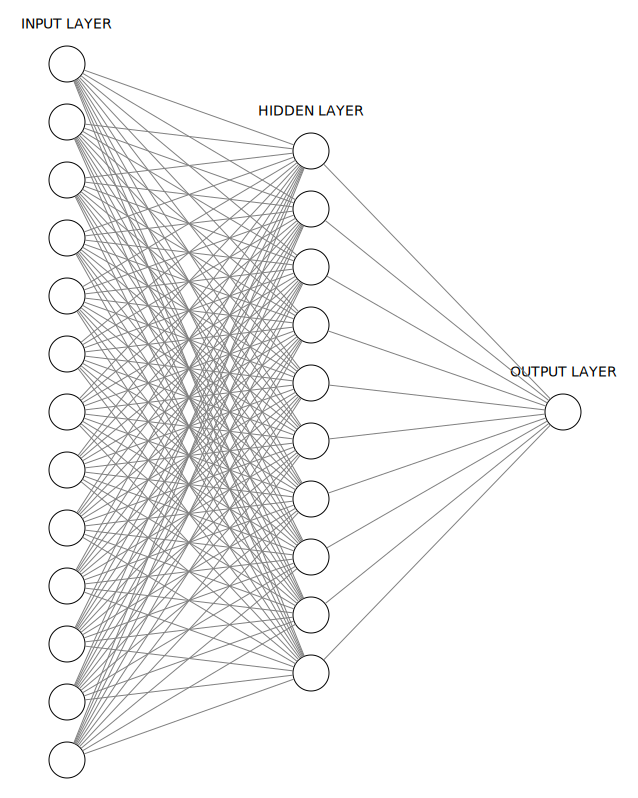
\includegraphics[width=.6\textwidth]{image/mlp.png}
	\caption{Representação gráfica da MLP com três camadas}
	\label{fig:mlp}
\end{figure}

\begin{figure}[h]
	\centering
	\includegraphics[width=.6\textwidth]{image/mlp2.png}
	\caption{Representação gráfica da MLP com três camadas}
	\label{fig:mlp2}
\end{figure}

%O funcionamento da MLP é dividido em duas fases: \textit{forward} e \textit{backward}. Na fase \textit{forward}, um neurônio de uma camada está ligado a todos os neurônios da camada seguinte. Os sinais da entrada são propagados da camada de entrada para a camada escondida e da camada escondida para a camada de saída; cada neurônio processa as entradas e apresenta uma saída. Nessa fase é possível calcular o erro entre a saída desejada para a rede e a saída apresentada pela MLP. Na fase \textit{backward} o erro é retropropagado e os pesos são ajustados, utilizando o algoritmo de ajustes de pesos, inicialmente aleatórios, chamado \textit{Backpropagation} \cite{valenca2005aplicando}.
The operation of MLP is divided in two stages: forward and backward. In forward stage, a neuron of a layer is connected to all neurons in next layer. The input signals are propagated from the input layer to the hidden layer and from the hidden layer to the output layer. Each neuron processes the inputs and provides an output. In that stage it is possible to calculate the error between the desired output to the network and the output presented by MLP. In the backward phase, the error is backpropagated and weights are adjusted using the algorithm of weight adjustment, initially random, called Backpropagation \cite{valenca2005aplicando}.

\subsubsection{Backpropagation Algorithm}

%A primeira etapa do \textit{Backpropagation} consiste na inicialização dos pesos com valores aleatórios. A partir daí, para cada exemplo da base de treinamento são realizados os seguintes passos: a propagação do sinal; a fase \textit{forward} e retropropagação do erro; e a fase \textit{backward}. Na fase \textit{forward} é possível calcular o erro entre a saída desejada para a rede e a saída apresentada pela MLP. Na fase \textit{backward} o erro é retropropagado e os pesos são ajustados. Faz-se necessário calcular a sensibilidade para cada neurônio. A sensibilidade para as camadas é dada por:
The first phase of Backpropagation consists on inicializing weights with ramdom values. Thereafter, for each example from training subset the following steps are performed: signal propagation, forward phase and error backpropagation, backward phase. In forward phase it is possible to calculate the error between expected and calculated outcome, from MLP network. In backward phase error is backpropagated and weights are adjusted. It is necessary to calculate sensibility for each neuron. Sensibility for each layer is given by:

\begin{equation}
\label{eq:sensibiliy_function}
\delta^{m-1}_i = f^{m-1'}(net^{m-1}_j)\sum_{i=1}^{N_{neurons}}w^m_{ij}\delta^m_i
\end{equation}

%em que, $w^m_{ij}$ são os pesos sinápticos que serão ajustados, $\delta^m_i$ representa a sensibilidade, o índice $i$ representa o número de neurônios da camada que recebe o sinal e possui $N_{neurons}$ e $f^{m-1'}(net^{m-1}_j)$ é a derivada da função de ativação dos neurônios da camada "M-1" (camada que emite o sinal) em relação à entrada líquida, $net^{m-1}_j$.
where $w^m_{ij}$ are synaptic weights that will be adjusted, $\delta^m_i$ represents sensibility, index $i$ represents neuron numbers of the layer that receives the signal and has $N_{neurons}$, ending $f^{m-1'}(net^{m-1}_j)$ is the derivative of the activation function for neurons of layer "M-1" (the layer that emits signal) in relation to net input, $net^{m-1}_j$.

%O ajuste dos pesos é dado por:
Weight adjustment is given by:

\begin{equation}
\label{eq:backpropagation_function}
w^m_{ij}(t+1) = w^m_{ij}(t) + \alpha \delta^m_i y^{m-1}_j + \beta \Delta w^m_{ij}(t-1)   
\end{equation}

%em que $\alpha$ é a taxa de aprendizagem do algoritmo, $\beta$ é a taxa de momento e $\Delta w^m_{ij}(t-1)$ é a correção realizada no peso $w_{ij}^m$ na iteração $t-1$. Quanto maior o valor de $\alpha$ maiores serão as correções realizadas a cada iteração. Já o momento $\beta$ tem o objetivo de deixar o algoritmo menos susceptível a ficar preso em mínimos locais (no algoritmo original,$\beta = 0$), devido a superfície da função erro ser bastante complexa.
where $\alpha$ is the algorithm learning rate, $\beta$ is the moment and $\Delta w^m_{ij}(t-1)$ is the correlation to weight $w_{ij}^m$ in iteration $t-1$. The higher $alpha$ value the higher will be correlations performed in each iteration. $\beta$ moment aim to making the algorithm less susceptible to getting trapped in local minima (in the original  algorithm, $\beta = 0$), due to the surface of the error function be fairly complex.

%Durante o treinamento as entradas vão sendo apresentados à MLP de forma aleatória e os pesos vão sendo ajustados pelo algoritmo \textit{backprogation} até que se chegue a uma condição de parada. A parada do treinamento é uma decisão crítica, pois uma parada prematura do treinamento poderá acarretar o \textit{underfitting} (os pesos da MLP não são ajustados de forma satisfatória), e caso o treinamento se torne excessivamente longo, pode ocorrer o \textit{overfitting} (a rede memoriza os exemplos de treinamento e ocorre perda na capacidade de generalização) \cite{valenca1995fundamentos}. Objetivando evitar essas duas condições, e consequentemente uma melhor capacidade de generalização, a base de dados para treinamento da rede pode ser dividida em duas partes: uma parte de fato para treinamento e uma outra parte para validação. O subconjunto para treinamento é apresentada à rede e serve para realizar o ajuste dos pesos pelo algoritmo de treinamento. O subconjunto de validação serve para realizar uma avaliação do treinamento da rede. Quando a REMQ para o subconjunto de validação começar a aumentar, significa que a MLP está memorizando o conjunto de treinamento e neste momento é adequado interromper o treinamento.
During training, inputs are being presented to MLP randomly and the weights are being adjusted by backpropagation algorithm until reaches stop condition. The training stop is a critical decision because a premature stop in training can lead to underfitting (where weights of the MLP are not adjusted satisfactorily), and if the training becomes excessively long it can lead to overfitting (where the network memorizes the training examples and loss occurs in generalizability) \cite{valenca1995fundamentos}. Aiming avoiding these two conditions, and consequently a better generalization capability, the training data set of the network can be divided in two parts: one subset for training in fact, and another for validation. Training subset is presented to the network and serves to make weight adjustments through training algorithm. validation subset serves to perform an training assessment. When REMQ of validation subset starts to increase, means that MLP is memorizing training subset and at this is appropriated interrupt the training.

%As redes MLP são uma boa ferramenta para a construção de classificadores, já que além de conseguir lidar com o mapeamento entrada-saída não linear, apresentam alto poder de generalização \cite{haykin-1994}.
MLP networks are a good approach for building classifiers, since besides coping with input-output nonlinear mapping, they have high power of generalization \cite{haykin-1994}.

%Em \cite{HUHUANG2007}, algumas técnicas inteligentes são utilizadas para a análise do risco de projetos de software. O artigo conclui que uma técnica híbrida de redes neurais e algoritmos genéticos obtém uma precisão de 85\% na previsão do projeto obter sucesso, ser desafiado ou falhar totalmente.
In \cite{HUHUANG2007}, some clever techniques are utilized for risk analysis software projects. The paper concludes that a hybrid technique of neural networks and genetic algorithms achieved an accuracy of 85\% to predict whether the project will succeed, fail completely or will be challenged.

\subsection{Support Vector Machine}

%A Máquina de Vetor de Suporte, do inglês \textit{Support Vector Machine} (SVM), é uma técnica de aprendizado de máquina aplicável a problemas de reconhecimento de padrões nos quais se busca atingir alto potencial de generalização \cite{HAYKIN2007} \cite{valenca2005aplicando}. O objetivo da SVM é encontrar um hiperplano particular, denominado de hiperplano ótimo, que maximize a margem de separação, conforme pode ser visualizado na Figura \ref{fig:svm}. Na Figura \ref{fig:svm}, observamos dois vetores de suporte capazes de separar linearmente as saídas no hiperplano em duas classes. A variável $r$ é a distância algébrica desejada dos vetores de suporte para o hiperplano ótimo de separação das classes. Quanto maior essa distância, maior a capacidade de generalização da máquina de vetor de suporte.
Support Vector Machine (SVM) is a machine learning technique applied to pattern recognition problems in which one seeks to achieve high generalization capability \cite{HAYKIN2007} \cite{valenca1995fundamentos}. The goal of SVM is to find a particular output hyperplane, called the optimal hyperplane that maximizes the margin of separation, as can be seen in Figure \ref{fig:svm}. In Figure \ref{fig:svm}, we observed two support vectors capable of linearly dividing output hyperplane into two classes. The variable $r$ is the desired algebraic distance from support vectors to the optimal hyperplane separating each class. The larger the distance, the higher the generalization ability in support vector machine.

\begin{figure}[h]
	\centering 
	\includegraphics[width=.6\textwidth]{image/svm.png}
	\caption{Vetores de Suporte e Hiperplano de Separação ótimo}
	\label{fig:svm}
\end{figure}

%As SVMs foram desenvolvidas tendo por base a teoria do aprendizado estatístico, detalhada por Vapnik em 1995 e 1998 \cite{vapnikSnature} \cite{vapnik1998statistical}, e inicialmente proposta por Vapnik e Chervonenkis em 1971 \cite{vapnik1971uniform}.
SVMs were developed based on statistical learning theory, detailed by Vapnik in 1995 and 1998 \cite{vapnikSnature} \cite{vapnik1998statistical}, and initially proposed by Vapnik and Chervonenkis in 1971 \cite{vapnik1971uniform}.

%O desenvolvimento das SVMs teve por objetivo obter algoritmos com alta capacidade de generalização. De acordo com a teoria do aprendizado estatístico este erro de generalização chamado de Risco Funcional pode ser calculado caso se conheça a distribuição de probabilidade da população \cite{vapnik1998statistical}. Entretanto, para problemas de aprendizado supervisionado, em geral não se dispõe da distribuição de probabilidade da população,uma vez que em problemas reais o que se utiliza é uma amostra da população sendo possível apenas o cálculo de uma função erro, como por exemplo o erro médio quadrático. Esta função erro calculada da amostra de dados é chamada de Risco Empírico. Logo, a depender do tamanho da amostra utilizada para treinamento, a minimização do erro de treinamento, não significa necessariamente uma minimização do erro de generalização ou Risco Funcional.
The development of SVMs aimed to obtain algorithms with high generalization capability. According to the theory of statistical learning this generalization error called Functional Risk can be calculated if one knows the probability distribution of the population \cite{vapnik1998statistical}. However, for supervised learning problems generally the probability distribution of the population is not available, since in real problems it is used a population sample. Therefore it is only possible to calculate an error function, such as REMQ. This error function calculated from the sample data is called Empirical Risk. Depending on the sample size used for training, minimizing the training error does not necessarily mean minimizing the generalization error or Functional Risk.

%Um conceito importante da teoria do aprendizado estatístico é o da dimensão VC (Vapnik-Chervonenkis). A dimensão VC é um índice escalar que mede a complexidade intrínseca de uma classe de funções. Uma definição para a dimensão VC é de que esta representa o número máximo de exemplos de treinamento que uma máquina de aprendizagem é capaz de classificar corretamente, para todas as possíveis combinações binárias desses dados.
An important concept in statistical learning theory is the VC dimension (Vapnik-Chervonenkis). The VC dimension is a scale index that measures the intrinsic complexity of a class of functions. A definition of the VC dimension is that this represents the maximum number of training examples that a machine learning is able to correctly classify, for all possible binary combinations of these data.

%Desta forma, de acordo com a teoria do aprendizado estatístico proposta por Vapnik \cite{vapnik1998statistical}, uma rede neural ou qualquer outra máquina de aprendizagem durante o aprendizado supervisionado obtém sua capacidade máxima de generalização quando durante o treinamento se minimiza o Risco Funcional. A minimização do Risco Funcional é equivalente a minimização do Risco Empírico e do Risco Estrutural associado a complexidade do modelo. O Risco Funcional é limitado, com probabilidade $1 - \delta$ pela Equação \ref{eq:svm_functional_risk}.
Thus, according to the statistical learning theory proposed by Vapnik \cite{vapnik1998statistical}, a neural network or any other machine learning during the supervised learning obtains its maximum capacity of generalization when during training it minimizes the functional risk. Minimising Functional Risk is equivalent to minimize empirical risk and structural risk associated with model complexity. The Functional Risk is limited, with probability $1 - \delta$ by Equation \ref{eq:svm_functional_risk}.

\begin{equation}
\label{eq:svm_functional_risk}
R_{funcional} \leq R_{empirico} + R_{estrutural}
\end{equation}

%O Risco Estrutural por sua vez pode ser calculado, conforme mostrado por Vapnik \cite{vapnik1998statistical} como:
The Structural Risk can be calculated, as shown by Vapnik \cite{vapnik1998statistical} as:

\begin{equation}
\label{eq:svm_structural_risk}
R_{estrutural} = \sqrt{\frac{h \left( \log \left( \frac{2N}{h} \right) + 1 \right) - \log \left( \frac{\delta}{4} \right)}{N}}
\end{equation}

%onde $h$ é a dimensão VC.
where $h$ is the dimension VC.

%A formulação inicial das SVMs para problemas linearmente separáveis foi chamada de SVMs de margens rígidas (máximas). A diferença destas para uma rede \textit{perceptron} está na forma de seleção do hiperplano de separação das classes. Enquanto numa rede \textit{perceptron} se busca qualquer hiperplano que satisfaça o problema, numa SVM de margem rígida se procura o hiperplano ótimo, ou seja, aquele cuja margem de separação é máxima.
The initial formulation of SMVMs for linearly separable problems was called rigid edges (maximum). The difference of these to a perceptron network is in the method of selecting the hyperplane that separates the classes. While a perceptron network seeks any hyperplane that satisfies the problem, a rigid margin SVM seeks the optimal hyperplane, ie, one whose margin of separation is maximum.

%Desta forma, a determinação dos pesos das SVMs se tranforma em um problema de otimização com restrição, o que exige um maior esforço computacional. A otimização dos pesos das SVMs com restrição de margem máxima tem sido resolvida através do método de multiplicadores de Lagrange.
This way, the determination of SVMs weights is transformed into a constrained optimization problem, which requires a higher computational effort. The optimization of the SVMs weights with restricted maximum margin has been solved by the method of Lagrange multipliers.

%Posteriormente, foram elaboradas as SVMs de margens flexíveis (suaves) com o objetivo de lidar com amostras de treinamento com erros ou ruídos e finalmente as SVMs não lineares que utilizam na camada escondida funções de base diferentes.
Subsequently, flexible margins SVMs were developed with the aim of dealing with the training samples with errors and finally the SVM using nonlinear functions in the hidden layer of different base.

%Para um melhor entendimento das SVMs considere um problema de classificação linear com vetor de entrada $x_i$ $(i=1,...,n)$, onde $n$ é o número de exemplos e saídas $y_i$ (+1 ou -1). A seleção dos parâmetros deve ocorrer de tal forma que:
For a better understanding of SVMs consider a linear classification problem with linear input vector  $x_i$ $(i=1,...,n)$, where $n$ is the number of examples and outputs $y_i$ (+1 ou -1). The selection of parameters should occur such that:

\begin{eqnarray}
\label{eq:svm_example}
w^T.x_i + b \geq +1 ,& se& y_i= +1 \\
w^T.x_i + b \leq -1 ,& se& y_i= -1 
\end{eqnarray}

%ou de forma resumida
or in summary

\begin{eqnarray}
\label{eq:svm_example_summary}
y_i (w^T.x_i + b) \geq 1 ,&& i=1,..,n
\end{eqnarray}

%A margem $d$ é a distância entre os dois planos paralelos e pode ser expressa como uma distância euclidiana, na Equação \ref{eq:svm_euclian_distance}.
Margin $d$ is the distance between two parallel planes and can be expressed as an euclidean distance in Equation \ref{eq:svm_euclian_distance}.

\begin{equation}
\label{eq:svm_euclian_distance}
d = \frac{| w^T.x_i + b |}{|| w ||} + \frac{| w^T.x_i + b |}{|| w ||} = \frac{2}{|| w ||}
\end{equation}

%onde, $||w|| = \sqrt{w_1^2 + w_2^2 + ... + w_n^2}$ é a norma Euclidiana do vetor de pesos.
where $||w|| = \sqrt{w_1^2 + w_2^2 + ... + w_n^2}$ is the euclidian norm of weights vector.

%Portanto, maximizar a margem se transforma em um problema de otimização com restrição para minimizar a seguinte função objetivo $\min_w \frac{||w||^2}{2}$ sujeito a Equação \ref{eq:svm_example_summary}.
Therefore, maximizing the margin becomes a constrained optimization problem to minimize the following objective function $\min_w \frac{||w||^2}{2}$ subject to Equation \ref{eq:svm_example_summary}.

%Esse é um problema de otimização não-linear (a função objetivo é quadrática) com restrições lineares que pode ser resolvido por meio dos multiplicadores de Lagrange.
This is a nonlinear optimization problem (the objective function is quadratic) with linear constraints which can be solved by means of Lagrange multipliers.

\subsection{Radial Basis Function Network}

%As Redes de Função de Base Radial \textit{Radial Basis Function }(RBF) surgiram em 1988 como uma possível alternativa às redes MLP. Na sua formulação tradicional é composta por três camadas: uma camada de entrada, uma camada escondida e uma camada de saída. As principais diferenças entre as redes RBF e MLP são:
Radial Basis Function (RBF) network emerged in 1988 as a possible alternative to MLP networks. In its traditional formulation is composed of three layers: an input layer, a hidden layer and an output layer. The main differences between the MLP and RBF networks are:

%\begin{enumerate}
%\item Os neurônios da camada intermediária têm apenas funções de base radial como função de ativação, que são funções localizadas de tal maneira que apenas algumas unidades escondidas ficarão ativadas ao receberem um dado conjunto de exemplos de entrada;
%\item Nas redes MLP as funções de ativação têm como entrada líquida uma média ponderada entre os exemplos de entrada e o conjunto de pesos. Por outro lado, nas redes RBF a utilização destas funções de ativação de base radial fazem com que sua ativação seja obtida a partir de uma norma ponderada da diferença entre o valor de entrada e o centro da função de base radial;
%\item A camada de saída é composta por unidades de processamento lineares.
%\end{enumerate}
\begin{enumerate}
\item The neurons in the hidden layer have only radial basis functions as activation functions, which are located in such a way that only a few hidden units will be activated when receiving a given set of input samples;
\item In MLP networks activation functions have as a weighted average net inflow among input samples and the set of weights.  On the other hand, in RBF networks the use of these activation functions of radial basis make it fired through a weighted norm of the difference between the input value and the radial basis function center;
\item The output layer is composed of linear processing units.
\end{enumerate}

%As funções de ativação mais utilizadas são \cite{valenca2005aplicando} \cite{engelbrecht2007computational}:
The most commonly used activation functions are \cite{valenca2005aplicando} \cite{engelbrecht2007computational}:

\begin{enumerate}
%\item Função Linear
\item Linear Function

\begin{equation}
\label{eq:rbf_linear_function}
\phi_i(x) = || x_j - \mu_i ||
\end{equation}

%\item Função Cúbica
\item Cubic Function

\begin{equation}
\label{eq:rbf_cubic_function}
\phi_i(x) = || x_j - \mu_i ||^3
\end{equation}

%\item Função de base Gaussiana
\item Gaussian Basis Function

\begin{equation}
\label{eq:rbf_gaussian_function}
\phi_i(x) = exp \left( - \frac{|| x_j - \mu_i ||^2}{2\sigma_{i}^{2}} \right)
\end{equation}

%\item Função Logística
\item Logistic Function

\begin{equation}
\label{eq:rbf_logistic_function}
\phi_i(x) = \frac{1}{1 + exp \left( - \frac{|| x_j - \mu_i ||^2}{\sigma_{i}^{2} - \theta} \right)}
\end{equation}

%\item Função de base Multi-quadrática
\item Multi-quadratic Basis Function

\begin{equation}
\label{eq:rbf_multiquadratic_function}
\phi_i(x) = \sqrt{|| x_j - \mu_i ||^2 + \sigma_i^2}
\end{equation}

%\item Função de base Multi-quadrática inversa
\item Inverse Multi-quadratic Basis Function

\begin{equation}
\label{eq:rbf_inverse_multiquadratic_function}
\phi_i(x) = \frac{1}{\sqrt{|| x_j - \mu_i ||^2 + \sigma_i^2}}   
\end{equation}

%\item Função de base lâmina de fina Spline
\item Thin Blade Spline Basis Function

\begin{equation}
\label{eq:rbf_spline}
\phi_i(x) = \frac{|| x_j - \mu_i ||}{\sigma_i^2} \log \left( \frac{|| x_j - \mu_i ||}{\sigma_i} \right)   
\end{equation}

\end{enumerate}

%onde, $x_j$ são amostras de entrada, $\mu_i$ e $\sigma_i$ representam respectivamente o centro e a largura (dispersão) da i-ésima função de base radial e $\theta$ é um bias ajustado.
where, $x_j$ are input samples, $\mu_i$ and $\sigma_i$ represents respectively the center and the width (dispersion) of the i-th radial basis function and $\theta$ is an adjusted bias.

%O cálculo da resposta da rede RBF correspondente aos neurônios da camada de saída é realizado pela Equação \ref{eq:rbf_output_formula}.
The calculation of the response of RBF corresponding to the neurons of the output layer is performed by Equation \ref{eq:rbf_output_formula}.

\begin{equation}
\label{eq:rbf_output_formula}
y_j = \sum_{j=1}^{s} w_{Kj} \phi_K(x)   
\end{equation}

%O treinamento das redes RBF pode ser realizado de diversas formas. Dentre as abordagens propostas, o treinamento mais empregado é chamado de treinamento híbrido, por utilizar uma aprendizagem não supervisionada para determinar os parâmetros das funções de base radial da camada escondida e um aprendizado supervisionado para ajustar os pesos que ligam a camada escondida a de saída. Portanto, desde que as funções de base radial, após determinação de seus parâmetros, sejam consideradas fixas, o ajuste dos pesos que ligam a camada escondida para a camada de saída para a rede RBF fica equivalente a uma rede ADALINE. Neste caso, ao se utilizar neurônios lineares na camada de saída e uma função objetivo como o erro médio quadrático, o treinamento destas redes é bastante rápido, uma vez que dispomos de um sistema de equações lineares para ser resolvido, o que nos permite utilizar técnicas lineares de inversão de matriz.
The training of RBF networks can be accomplished in several ways. Among the proposed approaches, the most adopted training is called hybrid training, because it uses an unsupervised learning to determine the parameters of radial basis functions of the hidden layer and supervised learning to adjust the weights that links the hidden layer to the output layer. Therefore, since the radial basis functions are considered fixed after determining its parameters, adjusting the weights that links the hidden layer to the output layer for the RBF network is equivalent to an ADALINE network. In this case, when using linear neurons in the output layer and an objective function such as mean square error, the training of these networks is very fast since we have a system of linear equations to be solved, which allows us to use linear techniques of matrix inversion.

%Durante a primeira fase de treinamento, aprendizagem não supervisionada, os centros das funções de base radial podem ser determinados por algoritmos de clusterização, tais como algoritmos k-médias \cite{musavi1992training} e mapas auto-organizáveis de Kohonen \cite{valenca1995fundamentos}.
During the first phase of training, unsupervised learning, the centers of radial basis functions can be determined by clustering algorithms such as k-means algorithm \cite{musavi1992training} and self-organized kohonen maps \cite{valenca1995fundamentos}.

%O método k-média tem por objetivo encontrar um conjunto de $K$ centros, $\mu_i$ (i=1,2,...,$K$), representativos das funções de base radial em função do conjunto de exemplos de entrada $x_j$ com $j=1,2,...,N$. O algoritmo divide o conjunto de entrada em K subconjuntos $S_i$ cada um deles contendo $N_i$ exemplos. O objetivo do método é minimizar a Equação \ref{eq:rbf_minimization_function}.
K-means method has the objective to find a set of $K$ representative centers, $\mu_i$ (i=1,2,...,$K$), of radial basis function in terms of input samples $x_j$ with $j=1,2,...,N$. The algorithm divides the input data set in $K$ subsets $S_i$ each one containing $N_i$ examples. The purpose of the method is to minimize Equation \ref{eq:rbf_minimization_function}.

\begin{equation}
\label{eq:rbf_minimization_function}
F = \sum_{i=1}^{K} \sum_{j \in S_i} || x_j-\mu_i ||^2
\end{equation}

%onde, $\mu_i$ é a média dos pontos pertencentes ao conjunto $S_i$ calculada por
where, $\mu_i$ is the mean of points belonging to $S_i$ set calculated by

\begin{equation}
\label{eq:rbf_mi_i}
\mu_i = \frac{1}{N_i} \sum_{j \in S_i} x_j
\end{equation}

%Inicialmente, os exemplos de entrada são localizados aleatoriamente dentro de cada subconjunto $K$ e então os centros $\mu_i$ são calculados. Posteriormente, os exemplos são redistribuídos de acordo com a sua maior proximidade com relação a estes centros. Este processo é então repetido até que não ocorram mais mudanças de exemplos entre os grupos. Este método permite também determinar o valor da largura (dispersão) $\sigma_i$ da função de base radial por meio da distância euclidiana.
Initially, the input samples are randomly located within each subset $K$ and then the centers $\mu_i$ are calculated. Subsequently, the samples are redistributed according to its closer proximity with regard to these centers. This process is then repeated until there are no more changes between the groups of examples. This method also allows to determine the value of the width (dispersion) $\sigma_i$ of radial basis function using the Euclidean distance.

%Logo, após a finalização do treinamento não-supervisionado onde foram determinados os parâmetros das funções de base radial, se realiza a segunda parte do treinamento que consiste em um treinamento supervisionado onde se determinam os pesos que ligam a camada escondida à camada de saída. Nessa fase, o treinamento é similar a uma rede tradicional com a utilização de uma função objetivo tal como o erro médio quadrático. Diversas técnicas de otimização podem ser utilizadas para o aprendizado dos pesos da camada de saída, responsáveis pela combinação linear das ativações da camada escondida, tais como: a regra delta, o método dos mínimos quadrados, a técnica de pseudo-inversão e o método OLS (\textit{Orthogonal Least Squares}) \cite{chen1991orthogonal}.
Soon after completion of the non-supervised training where it was determined the parameters of radial basis functions, is held the second part of the training that consists of a supervised training where the weights that links the hidden layer to the output layer are determined. In this phase, the training is similar to a traditional network with use of an objective function such as mean square error. Several optimization techniques can be used for learning the weights of the output layer, responsible for the activation of the linear combination of the hidden layer, such as the delta rule, the method of least squares technique pseudo-inversion and Orthogonal Least Squares (OLS).

%As redes RBF são aproximadores universais de função tal como a rede MLP. Em geral as redes RBF têm um tempo de treinamento inferior ao de uma rede MLP, uma vez que o treinamento híbrido da RBF permite a utilização de técnicas lineares de rápida convergência para determinação dos pesos (entre as camadas escondida e a de saída) durante o aprendizado supervisionado.
RBF networks are universal function approximators such as MLP. In general RBF networks have a training duration less than in MLP, since the hybrid RBF training techniques permits the use of linear fast convergence for determining the weights (between hidden and output layers) during supervised learning.

%As redes RBF por serem redes de aprendizado local, necessitam de uma quantidade maior de amostras para o seu treinamento, para que se obter uma precisão similar a das redes MLP, que são redes de ajuste global. Isto implica que as redes MLP em geral são melhores aproximadores de funções, pois o ajuste global tende a fornecer uma maior capacidade de generalização. Entretanto, em problemas de classificação, as redes MLP tendem a cometer maiores erros de classificação "falso positivo" do que as redes RBF \cite{valenca1995fundamentos}.
RBF networks such as local learning networks, require a larger number of samples for its training to obtain an accuracy similar to that MLP networks, which are networks of global adjustment. This implies that the MLP are usually better approximators of functions because the global adjustment tends to provide greater generalizability. However, in classification problems, the MLP tend to make greater misclassification "false positive" than RBF networks

\subsection{Learning Rules}

%Uma propriedade de importância primordial para uma rede neural é a sua habilidade de aprender a partir de seu ambiente e de melhorar o seu desempenho. A melhoria do desempenho ocorre com o tempo de acordo com alguma medida preestabelecida. Uma rede neural aprende acerca do seu ambiente através de um processo iterativo de ajuste de seus pesos sinápticos e níveis de bias. Idealmente, a rede se torna mais instruída sobre o seu ambiente após cada iteração do processo de aprendizagem.
A property of major importance for a neural network is its ability to learn from its environment and improve its performance. The improvement in performance occurs over time according to some predetermined measure. A neural network learns about its environment through an iterative process of adjusting its synaptic weights and bias levels. Ideally, the network becomes more educated about their environment after each iteration of the learning process.

\subsubsection{Gradient Descent Learning}

%O Gradiente Descendente (GD) requer a definição de uma função erro (ou objetivo) para medir o erro do neurônio na aproximação do alvo, a soma quadrática dos erros é normalmente usada \ref{eq:sse}. O objetivo do GD é encontrar os valores de peso que minimizem a função de erro obtido através do cálculo da inclinação da função de erro no espaço de pesos com o objetivo de mover o vetor de pesos ao longo do gradiente negativo, tal como ilustrado por um único erro na Figura \ref{fig:gd} \cite{engelbrecht2007computational}.
Gradient Descent (GD) requires the definition of an error (or objective) function to measure the neuron's error in approximating the target. The sum of square errors is usually used \ref{eq:sse}. The aim of GD is to find the weight values that minimizes the error function. This is achieved by calculating the gradient of the error function in weight space, and to move the weight vector along the negative gradient as illustrated for a single error in Figure \ref{fig:gd} \cite{engelbrecht2007computational}.

\begin{equation}
\label{eq:sse}
\epsilon = \sum\limits_{i=1}^{P_T}(e_i - c_i)^2
\end{equation}

%onde $e_i$ e $c_i$ são respectivamente a saída esperada e calculada para o i-ésimo padrão, e $P_T$ é o número total de pares de vetores entrada-saída no conjunto de treinamento.
where $e_i$ and $c_i$ are respectively the expected and calculated output for the i-th pattern, and $P_T$ is the total number of input-target vector pairs (\textit{patterns}) in the training set.

\begin{figure}[h]
	\centering
	\includegraphics[width=.6\textwidth]{image/gd.png}
	\caption{Vetores de Suporte e Hiperplano de Separação ótimo}
	\label{fig:gd}
\end{figure}

%Dado um padrão único de treinamento, os pesos são atualizados usando:
Given a single training pattern, weights are updated using 

\begin{equation}
\label{eq:gd1}
v_i(t) = v_i(t-1) + \Delta v_i(t)
\end{equation}

%onde
where

\begin{equation}
\label{eq:gd2}
\Delta v_i(t) = \eta (- \frac{\partial \epsilon}{\partial v_i})
\end{equation}

%e $\eta$ é a taxa de aprendizagem (isto é, o tamanho dos passos dados na direção contrária ao gradiente). A regra de aprendizagem Widrow-Hoff apresenta uma solução para as funções de passo e rampa, enquanto a regra de aprendizagem delta generalizada assume funções contínuas que sejam pelo menos diferenciáveis uma vez \cite{engelbrecht2007computational}.
and $\eta$ is the learning rate (i.e. the size of steps taken in the negative direction of the gradient). The Widrow-Hoff learning rule presents a solution for the step and ramp functions, while the generalized delta learning rule assumes continuous functions that are at least once differentiable \cite{engelbrecht2007computational}.

\subsubsection{Widrow-Hoff Learning}

%A regra de aprendizagem Widrow-Hoff assume que se a função objetivo $f = net_i$, então $\frac{\partial f}{\partial net_i}$. Essa regra de aprendizagem também é conhecida como o algoritmo \textit{least-mean-square} (LMS), foi um dos primeiros algoritmos usados para treinar redes neurais em camadas com múltiplos neurônios lineares adaptativos (Madaline) \cite{engelbrecht2007computational}.
Widrow-Hoff learning rule assumes that objective function $f = net_i$. Then $\frac{\partial f}{\partial net_i}$. This learning rule is also referred to as the least-mean-square (LMS) algorithm, was one of the first algorithms used to train layered neural networks with multiple adaptive linear neurons (Madaline) \cite{engelbrecht2007computational}.

\subsubsection{Error Correction Learning}

%A regra delta é uma generalização da regra de Widrow-Hoff \cite{widrow1960adaptive} que utiliza funções de ativação que tenham derivada real em todo seu domínio e ao menos um valor mínimo. A regra de aprendizagem é dada por:
Delta rule is a generalization of the Widrow-Hoff rule \cite{widrow1960adaptive} that uses activation functions that have real derivative throughout its domain and at least one minimum value. The learning rule is given by:

\begin{equation}
\label{eq:deltarule}
\Delta w_{ij} = \alpha(d_i - y_i)x_jf'(net_i)
\end{equation}

%ou seja, isso significa que o ajuste feito em um peso sináptico de um neurônio é proporcional ao produto do sinal de erro pelo sinal de entrada da sinapse em questão \cite{haykin-1994}. Assim, o ajuste a ser aplicado aos pesos é:
in other words, that means the adjustment made to a synaptic weight of a neuron is proportional to the product of the error signal by the input signal from the synapse in question \cite{haykin-1994}. Thus, the adjustment to be applied to the weights is:

\begin{equation}
\label{eq:peso_novo}
w_{ij}(new) = w_{ij}(old) + \alpha(d_i - y_i)x_jf'(net_i)
\end{equation}

%Esse algoritmo garante a minimização do erro ao longo do tempo, através do ajuste dos pesos, ou seja, sua convergência garante que a adaptação dos pesos seja realizada num número finito de iterações. A prova de convergência pode ser encontrada em Beale e Jackson \cite{beale2010neural}.
This algorithm ensures minimization of the error over time, by adjusting the weights, in other words, their convergence ensures that the adaptation of the weights is performed in a finite number of iterations. The proof of convergence can be found in Beale and Jackson \cite{beale2010neural}.

\subsubsection{Memory based Learning}

%Na aprendizagem baseada em memória, todas as (ou a maioria das) experiências passadas são armazenadas explicitamente em uma grande memória de exemplos de entrada-saída classificados corretamente: $ \{ ( x_i, d_i ) \}^{N}_{i=1}$, onde $x_i$ representa um vetor de entrada e $d_i$ representa a resposta desejada correspondente. Sem perda de generalidade, pode-se restringir a resposta desejada a um escalar. Em um problema de classificação de padrões binário, por exemplo, há duas classes/hipóteses a serem consideradas, representadas por $\zeta_1$ e $\zeta_2$. Neste exemplo, a resposta desejada $d_i$ assume o valor 0(ou -1) para a classe $\zeta_1$ e o valor 1 para a classe $\zeta_2$. Quando se deseja classificar um vetor de teste $x_teste$ (não visto antes), o algoritmo responde buscando e analisando os dados de treinamento em uma "vizinhança local" de $x_teste$.
In memory-based learning, all (or most of) previous experiences are explicitly stored in a large memory input-output examples classified correctly: $ \{ ( x_i, d_i ) \}^{N}_{i=1}$, where $x_i$ represents an input vector and $d_i$ is the corresponding desired response. Without loss of generality, one may restrict the desired response to a scalar. In a classification problem of binary patterns, for example, there are two classes/hypotheses to be considered, represented by $\zeta_1$ e $\zeta_2$. In this example, the desired response $d_i$ is set to 0 (or -1) for the class $\zeta_1$ and 1 for the class $\zeta_2$. When you want to classify a test vector $x_teste$ (not seen before), the algorithm responds searching and analyzing training data in a "local neighborhood" of $x_teste$.

%Todos os algoritmos de aprendizagem baseada em memória envolvem dois ingredientes essenciais:
Every learning algorithms based on memory involves two essential ingredients:

%\begin{enumerate}
%\item O critério utilizado para definir a vizinhança local do vetor de teste $x_teste$;
%\item A regra de aprendizagem aplicada aos exemplos de treinamento na vizinhança local de $x_teste$.
%\end{enumerate}
\begin{enumerate}
\item The criterion used to define the local neighborhood of the test vector $x_teste$;
\item The learning rule applied to the training samples in the local neighborhood $x_teste$.
\end{enumerate}

%Em um tipo mais efetivo de aprendizagem baseada em memória conhecido como a regra do vizinho mais próximo, a vizinhança local é definida como o exemplo de treinamento que se encontra na vizinhança imediata do vetor de teste $x_teste$. Em particular, diz-se que o vetor
On a more effective type of memory based learning known as the rule of the nearest neighbor, the local neighborhood is defined as the training example that is in the immediate vicinity of the test vector $x_teste$. In particular, it is said that the vector

\begin{equation}
\label{eq:nearestneighborhood_vector}
x'_N \in \{x_1, x_2, ..., x_N\},
\end{equation}

%é o vizinho mais próximo de $x_teste$ se 
is the nearest neighbor of $x_teste$ of

\begin{equation}
\label{eq:nearestneighborhood}
\min_i d(x_i, x_teste) = d(x'_N,x_teste),
\end{equation}

%onde $d(x_i, x_teste)$ é a distância euclidiana entre os vetores $x_i$ e $x_teste$. A classe associada com a distância mínima, ou seja, o vetor $x'_N$ é apresentada como a classificação de $x_teste$. Esta regra é independente da distribuição fundamental responsável pela geração dos exemplos de treinamento.
where $d(x_i, x_teste)$ is the euclidean distance between vectors $x_i$ and $x_teste$. The associated class with the minimum distance, that means, the vector $x'_N$ is displayed as classification $x_teste$. This rule is independent of the fundamental distribution responsible for generating training samples.

\subsubsection{Scaled Conjugate Gradient}

%A otimização do gradiente conjugado oferece uma escolha entre a simplicidade do gradiente descendente e a rápida convergência quadrática do método de Newton. Vários algoritmos de aprendizagem do gradiente conjugado foram desenvolvidos, a maioria deles são baseados no pressuposto de que a função de erro de todos os pesos da região de solução pode ser aproximada com precisão pela Equação \ref{eq:scg1} \cite{engelbrecht2007computational}:
Conjugate gradient optimization trades off the simplicity of GD and the fast quadratic convergence of Newton's method. Several conjugate gradient learning algorithms have been developed, most of which are based on the assumption that the error function of all weights in the region of the solution can be accurately approximated by  Equação \ref{eq:scg1} \cite{engelbrecht2007computational}:

\begin{equation}
\label{eq:scg1}
\varepsilon_T(D_T,w) = \frac{1}{2}w^THw - \theta^Tw
\end{equation}

%onde $H$ é a matriz Hessiana. Desde que a dimensão da matriz Hessiana seja o número total de pesos na rede, o cálculo das direções conjugadas na superfície de erro torna-se computacionalmente inviável. Algoritmos de gradiente conjugado computacionalmente viáveis calculam as direções do gradiente conjugado sem explicitamente computar a matriz Hessiana, e realizam atualizações nos pesos ao longo dessas direções.
where $H$ is the Hessian matrix. Since the dimension of the Hessian matrix is the total number of weights in the network, the calculation of conjugate directions on the error surface becomes computationally infeasible. Computationally feasible conjugate gradient algorithms compute conjugate gradient directions without explicitly computing the Hessian matrix, and perform weight updates along these directions.

%Um aspecto importante nos métodos de gradiente conjugado são os vetores de direção $\{p(0),p(1),...,p(t-1)\}$. Esses vetores são criados para ser conjugados com o vetor de pesos $w$. Isto é,  $p^T(t_1)wp(t_2) = 0$ para $ t_1 \neq t_2$. Um novo vetor de direção é gerado a cada iteração pela adição do vetor de gradiente negativo calculado, da função de erro, a uma combinação linear dos vetores de direção anteriores. O algoritmo de gradiente conjugado padrão assume uma função de erro quadrática, nos casos em que os algoritmos convergem em não mais que $n_w$ passos, onde $n_w$ é o número total de pesos e vieses. O algoritmo do gradiente conjugado Fletcher-Reeves não assume uma função de erro quadrática. O algoritmo é reiniciado após $n_w$ iterações se ainda não foi encontrada uma solução \cite{engelbrecht2007computational}.
An important aspect in conjugate gradient methods is that of direction vectors, $\{p(0),p(1),...,p(t-1)\}$. These vectors are created to be conjugated with the weight vector $w$. That is, $p^T(t_1)wp(t_2) = 0$ for $ t_1 \neq t_2$. A new conjugate direction vector is generated at each iteration by adding to the calculated current negative gradient vector of the error function a linear combination of the previous direction vectors. The standard conjugate gradient algorithm assumes a quadratic error function, in which case the algorithm converges in no more than $n_w$ steps, where $n_w$ is the total number of weights and biases. The Fletcher-Reeves conjugate gradient algorithm does not assume a quadratic error function. The algorithm restarts after $n_w$ iterations if a solution has not yet been found \cite{engelbrecht2007computational}.

%Os fatores de escala também pode ser calculado através de métodos Polak-Ribiere e Hestenes-Stiefer. Moller \cite{moller1993scaled} propôs o algoritmo de gradiente conjugado escalonado (GCS) como um algoritmo de aprendizado \textit{batch}. Os tamanhos do passo são determinados automaticamente e o algoritmo é reiniciado após $n_w$ iterações se uma boa solução não foi encontrada.
The scale factors can also be calculated through Polak-Ribiere and Hestenes-Stiefer methods. Moller \cite{moller1993scaled} proposed the scaled conjugate gradient (SCG) algorithm as a batch learning algorithm. Step sizes are automatically determined, and the algorithm is restarted after $n_w$ iterations if a good solution was not found.

\subsubsection{Quasi-Newton Learning}

%As variações em algoritmos de minimização são o gradiente e a matriz Hessiana. O gradiente deve ser conhecido com precisão assim como as direções de descidas devem ser calculadas a partir delas mesmas e aproximações ao gradiente não oferecem a precisão necessária. Por outro lado, a matriz Hessiana pode ser aproximada pela técnica das secantes. Uma vez que a matriz Hessiana é a matriz Jacobiana de um sistema de equações não-lineares $\nabla F(x) = 0$, ela pode ser aproximada. porém, a matriz Hessiana tem duas propriedades importantes: ela é sempre simétrica e, frequentemente, positiva. A incorporação dessas duas propriedades na aproximação secante é um aspecto importante dos métodos \textit{Broyden-Fletcher-Goldfarb-Shanno back-propagation} (BFGS-BP) e \textit{One Step Secant back-propagation} (OSS-BP) discutidos adiante. Eles são mais frequentemente chamados de atualizações secantes positivas definidas \cite{saini2002artificial}.
The derivatives in minimization algorithms are the gradient and the Hessian. The gradient must be known accurately as descent directions have to be calculated from them and approximations to gradient do not provide the required accuracy. On the other hand, the Hessian can be approximated by secant techniques. Since the Hessian is the Jacobian of the nonlinear system of equations $\nabla F(x) = 0$, it could be approximated. But, the Hessian has two important properties: it is always symmetric and often positive definite. The incorporation of these two properties into the secant approximation is an important aspect of the BFGS-BP and OSS-BP methods discussed subsequently. They are most often called positive definite secant updates \cite{saini2002artificial}.

\subsubsection{Broyden-Fletcher-Goldfarb-Shanno back-propagation method}

%No método de Newton uma aproximação quadrática é utilizada ao invés de uma aproximação linear da função $F(x)$. A próxima solução aproximada é obtida num ponto que minimize a função quadrática na Equação \ref{eq:bfgs1}.
In Newton's method a quadratic approximation is used instead of a linear approximation of the function $F(x)$. The next approximate solution is obtained at a point that minimizes the quadratic function in the Equação \ref{eq:bfgs1}.

\begin{equation}
\label{eq:bfgs1}
F(x_{k+1}) = F(x_k + \Delta x_k) = F(x_{k})+ g^T_k\Delta x_k + \frac{1}{2}\Delta x^T_k A_k \Delta x_k
\end{equation}

%Assim, a sequência obtida é a Equação \ref{eq:bfgs2}.
Hence, the obtained sequence is the Equation \ref{eq:bfgs2}.

\begin{equation}
\label{eq:bfgs2}
x_{k+1} = x_k - A^{-1}_k g_k
\end{equation}

%A principal vantagem do método de Newton é que ele tem uma taxa de convergência quadrática, enquanto que o descendente mais acentuada tem uma taxa de convergência linear, que é muito mais lento. No entanto, cada passo do método de Newton requer uma grande quantidade de computação. Supondo-se que a dimensionalidade do problema é N, uma operação de ponto flutuante O($N^3$) é necessária para calcular a direção da busca $d^k$.  Um método que utiliza uma matriz Hessiana aproximada para o cálculo da direção de busca é o método quasi-Newton. Seja  $H_k$ uma matriz simétrica $N \times N$ que aproxima a matriz Hessiana $A_k$; então a direção da pesquisa para o método quasi-Newton é obtida pela minimização da função quadrática, descrita pela Equação \ref{eq:bfgs3} \cite{saini2002artificial}.
The main advantage of the Newton's method is that it has a quadratic convergence rate, while the steepest descent has a much slower, linear convergence rate. However, each step of Newton's method requires a large amount of computation. Assuming that the dimensionality of the problem is N, an O($N^3$) floating-point operation is needed to compute the search direction $d^k$. A method that uses an approximate Hessian matrix in computing the search direction is the quasi-Newton method. Let $H_k$ be an $N \times N$ symmetric matrix that approximates the Hessian matrix $A_k$; then the search direction for the quasi newton-Newton method is obtained by minimizing the quadratic function, described by Equation \ref{eq:bfgs3} \cite{saini2002artificial}

\begin{equation}
\label{eq:bfgs3}
F(x_{k+1}) = F(x_{k})+ g^T_k\Delta x_k + \frac{1}{2}\Delta x^T_k H_k \Delta x_k
\end{equation}

%À medida que a matriz $H_k$ é aproximada à matriz Hessiana da função $F(x)$ em $x = x_k$, ela precisa ser atualizada a cada iteração, incorporando as informações de gradiente mais recentes \cite{saini2002artificial}.
As the matrix $H_k$ is to approximate the Hessian of the function $F(x)$ at $x = x_k$, it needs to be updated from iteration to iteration by incorporating the most recent gradient information \cite{saini2002artificial}.

\subsubsection{One-step Secant backpropagation method}

%Uma desvantagem da atualização do BFGS-BP na Equação \ref{eq:bfgs3} é que ela requer o armazenamento para uma matriz de tamanho $N \times N$ e cálculos de ordem O($N^ 2$). Apesar do armazenamento disponível ser um problema menor agora do que foi a uma década atrás, o problema computacional ainda existe para um grande valor de $N$. É possível usar uma aproximação secante com computação de O($N$). Nesse método, a nova direção de busca é obtida a partir de vetores calculados dos gradientes. Se $g_{k+1}$ é o gradiente atual, a nova direção de busca $p_{k+1}$ é obtida a partir da Equação \ref{eq:oss1} \cite{saini2002artificial},
One drawback of the BFGS update of Equation \ref{eq:bfgs3} is that it requires storage for a matrix of size $N \times N$ and calculations of order O($N^ 2$). Although the available storage is less of a problem now than it was a decade ago, the computational problem still exists for large $N$. It is possible to use a secant approximation with O($N$) computing. In this method, the new search direction is obtained from vectors computed from gradients. If $g_{k+1}$ is the current gradient, the new search direction $p_{k+1}$ is obtained as the Equation \ref{eq:oss1} \cite{saini2002artificial},

\begin{equation}
\label{eq:oss1}
p_{k+1} = - p_{k+1} + B_k y_k +C_k s_k
\end{equation}

%onde $g_{k+1} = \nabla F(x_{k+1})$ e os dois escalares $B_k$ e $C_k$ são a combinação dos produtos escalares dos vetores definidos anteriormente $s_k, g_{k+1}$ e $y_k$ (último passo, gradiente atual e diferenças dos gradientes)
where $g_{k+1} = \nabla F(x_{k+1})$ and the two scalars $B_k$ and $C_k$ are the following combination of scalar products of the previously defined vectors $s_k, g_{k+1}$ and $y_k$ (last step, current gradient and difference of gradients)

\begin{equation}
\label{eq:oss2}
B_k = \frac{s^T_k g_{k+1}}{s^T_k y_k}
\end{equation}

%e
and

\begin{equation}
\label{eq:oss3}
C_k = 1 \left(1 + \frac{y^T_k y_k}{s^T_k y_k} \right)  \frac{s^T_k g_{k+1}}{s^T_k y_k} + \frac{y^T_k g_{k+1}}{s^T_k y_k} .
\end{equation}

%A linha de busca de \textit{backtracking} é utilizada como o algoritmo de otimização do quasi-Newton do OSS-BP. No início do aprendizado, a direção de busca é $-g_0$ e é reiniciada para $-g_{k+1}$ a cada $N$ passos. O multiplicador $\left(1 + \frac{y^T_k y_k}{s^T_k y_k} \right)$ aumenta a última taxa de aprendizado que obteve sucesso e o primeiro passo da tentativa é executado.  Se a energia da rede é maior do que o valor limite superior, então uma nova tentativa é experimentada por meio de interpolação quadrática sucessiva até que a exigência seja cumprida. A taxa de aprendizagem é reduzida à metade após cada tentativa mal sucedida \cite{saini2002artificial}.
The backtracking line search is used with the quasi-Newton's OSS optimization algorithm. At the beginning of learning, the search direction is $-g_0$ and it is restarted to $-g_{k+1}$ every $N$ steps. The multiplier increases the last successful learning rate and first tentative step is executed. If the energy of the network is higher than the upper limiting value, then a new tentative is tried by using successive quadratic interpolation until the requirement is met. The learning rate is decreased to half after each unsuccessful trial \cite{saini2002artificial}.

\subsubsection{Levenberg-Marquardt Algorithm}

%O Algoritmo de Levenberg-Marquardt adaptativamente varia as atualizações de parâmetros entre a atualização do gradiente descendente e a atualização de Gauss-Newton \cite{marquardt1963algorithm},
The Levenberg-Marquardt algorithm adaptively varies the parameter updates between the gradient descent update and the Gauss-Newton update \cite{marquardt1963algorithm},

\begin{equation}
\label{eq:scg}
\varepsilon_T(D_T,w) = \frac{1}{2}w^THw - \theta^Tw
\end{equation}

%onde pequenos valores de parâmetros do algoritmo $\lambda$ resulta em uma atualização Gauss-Newton e grandes valores de $\lambda$ resultam numa atualização do gradiente descendente. O parâmetro $\lambda$ é inicializado para ser grande. Se uma iteração acontece de resultar numa aproximação pior, $\lambda$ é aumentado. À medida que a solução se aproxima do mínimo, $\lambda$ é diminuído, assim o método de Levenberg-Marquardt se aproxima do método de Gauss-Newton, e a solução tipicamente converge rapidamente para o mínimo local \cite{marquardt1963algorithm}.
where small values of the algorithm parameter $\lambda$ result in a Gauss-Newton update and large values of $\lambda$ result in a gradient descent update. The parameter $\lambda$ is initialized to be large. If an iteration happens to result in a worse approximation, $\lambda$ is increased. As the solution approaches the minimum, $\lambda$ is decreased, the Levenberg-Marquardt method approaches the Gauss-Newton method, and the solution typically converges rapidly to the local minimum \cite{marquardt1963algorithm}.

%O algoritmo sugeriu uma relação de atualização como na Equação \ref{eq:LMupdate}.
Marquardt’s suggested update relationship in Equation \ref{eq:LMupdate}.

\begin{equation}
\label{eq:LMupdate}
\varepsilon_T(D_T,w) = \frac{1}{2}w^THw - \theta^Tw
\end{equation}

\section{Neuro-Fuzzy Systems}

\subsection{ANFIS: Adaptive Neuro-Fuzzy Inference Systems}

%Nesta seção, apresentamos uma classe de redes adaptativas que são funcionalmente equivalentes aos sistemas de inferência Fuzzy, analisados durante esse estudo. A arquitetura é denominada como ANFIS, que significa \textit{Adaptive Network-based Fuzzy Inference System} ou semanticamente equivalente, Sistema de Inferência Neuro-fuzzy Adaptativo. Nós descrevemos como decompor o conjunto de parâmetros para facilitar a regra de aprendizagem híbrida para arquiteturas ANFIS representando os modelos fuzzy de Sugeno e Tsukamoto. Também demonstramos que, sob certas pequenas restrições, a Rede com Função de Base Radial é funcionalmente equivalente a arquitetura ANFIS para o modelo fuzzy de Sugeno \cite{jang1997neuro}.
In this section, we present a class of adaptive networks that are functionally equivalent to fuzzy inference systems, analyzed during this study. The architecture is referred to as ANFIS, which stands for adaptive network-based fuzzy inference system or semantically equivalently, adaptive neuro fuzzy inference system. We describe how to decompose the parameter set to facilitate the hybrid learning rule for ANFIS architectures representing both the Sugeno and Tsukamoto fuzzy models. We also demonstrate that under certain minor constraints, the radial basis functioin network (RBFN) is functionally equivalent to the ANFIS architecture for the Sugeno fuzzy model \cite{jang1997neuro}.

\begin{figure}[h]
	\centering
	\includegraphics[width=.7\textwidth]{image/anfis.png}
	\caption{(a) A two-input first-order Sugeno fuzzy model with two rules; (b) equivalent ANFIS architecture.}
%	\caption{(a) Um modelo fuzzy de Sugeno de primeira ordem com duas entradas e duas regras; (b) arquitetura equivalente ANFIS}
	\label{fig:anfis}
\end{figure}

\subsubsection{ANFIS Architecture}

%Por simplicidade, nós assumimos que o sistema de inferência fuzzy em consideração tem duas entradas $x$ e $y$ e uma saída $z$. Para um modelo fuzzy de Sugeno de primeira ordem, um conjunto de regras comum com duas regras fuzzy if-then são as sequintes:
For simplicity, we assume that the fuzzy inference system under consideration has two inputs $x$ and $y$ and one output $z$. For a first-order Sugeno fuzzy model, a common rule set with two fuzzy if-then rules is the following:

%\begin{enumerate}
%\item Regra 1: Se $x$ é $A_1$ e $y$ é $B_1$, então $f_1 = p_1x + q_1y + r_1,$
%\item Regra 2: Se $x$ é $A_2$ e $y$ é $B_2$, então $f_2 = p_2x + q_2y + r_2.$
%\end{enumerate}
\begin{enumerate}
\item Rule 1: If $x$ is $A_1$ and $y$ is $B_1$, then $f_1 = p_1x + q_1y + r_1,$
\item Rule 2: If $x$ is $A_2$ and $y$ is $B_2$, then $f_2 = p_2x + q_2y + r_2.$
\end{enumerate}

%A Figura \ref{fig:anfis}(a) ilustra o mecanismo de raciocínio para esse modelo de Sugeno; a arquitetura ANFIS equivalente correspondente é como mostrada na Figura \ref{fig:anfis}(b), em que nós da mesma camada têm funções similares, como descrito a seguir (Aqui definimos a saída do i-ésimo nó na camada $l$ como $O_{1,i}$).
Figure \ref{fig:anfis}(a) ilustrates the reasoning mechanism for this Sugeno model; the corresponding equivalent ANFIS architecture is as shown in Figure \ref{fig:anfis}(b), where nodes of the same layer have similar functions, as described next (Here we denote the output of the i-ésimo node in layer $l$ as $O_{1,i}$).

%\textbf{Camada 1}: Cada nó $i$ nessa camada é um nó adaptativo com um função:
\textbf{Layer 1}: Every node $i$ in this layer is an adaptive node with a node function

\begin{equation}
\label{eq:layer1anfis}
O_{1,i} = \mu_{A_i}(x), for i = 1,2 or \\
O_{1,i} = \mu_{B_{i-2}}(y), for i = 3,4
\end{equation}

%em que $x$ (ou $y$) é a entrada para o nó $i$ e $A_i$ (ou $B_{i-2}$) é um rótulo linguístico (tal como "pequeno" ou "grande") associado a esse nó. Em outras palavras, $O_{1,i}$ é o grau de pertinência a um conjunto fuzzy $A (A_1, A_2, B_1 or B_2)$ e ele especifica o grau em que a entrada de dados $x$ (ou $y$) satisfaz o quantificador $A$. Aqui, a função de pertinência para $ A $ pode ser qualquer função de pertinência parametrizada apropriada, como a função sino generalizada \cite{jang1997neuro}:
where $x$ (or $y$) is the input to node $i$ and $A_i$ (or $B_{i-2}$) is a linguistic label (such as "small" or "large") associated with this node. In other words, $O_{1,i}$ is the membership grade of a fuzzy set $A (A_1, A_2, B_1 or B_2)$ and it specifies the degree to which the given input $x$ (or $y$) satisfies the quantifier $A$. Here the membership function for $A$ can be any appropriate parameterized membership function, such as the generalized bell function \cite{jang1997neuro}:

\begin{equation}
\label{eq:bell_anfis}
\mu_{A}(x) = \frac{1}{1 + \left\| \frac{x - c_i}{a_i} \right\|^{2b}},
\end{equation}

%\textbf{Camada 2}: Cada nó nessa camada é um nó fixo rotulado $\Pi$, cuja saída é o produto de todos os sinais de entrada:
\textbf{Layer 2}: Every node in this layer is a fixed node labeled $\Pi$, whose output is the product of all the incoming signals:

\begin{equation}
\label{eq:layer2anfis}
O_{2,i} = w_i = \mu_{A_i}(x)\mu_{B_i}(y) for i = 1,2.
\end{equation}

%Cada nó saída representa a força de disparo de uma regra. Em geral, quaisquer outros operadores de norma T que executam a operação fuzzy "E" podem ser usados como função de nó nessa camada.
Each node output represents the firing strength of a rule. In general, any other T-norm operators that perform fuzzy AND can be used as the node function in this layer.

%\textbf{Camada 3}: Cada nó nessa camada é um nó fixo rotulado $N$. O i-ésimo nó calcula a taxa i-ésima força de disparo da regra para a soma de todas as forças de disparo das regras:
\textbf{Layer 3}: Every node in this layer is a fixed node labeled $N$. The i-th node calculates the ratio of the ith rule's firing strength to the sum of all rules' firing strengths:

\begin{equation}
\label{eq:layer3anfis}
O_{3,i} = \overline{w_i} = \frac{w_i}{w_1 + w_2} for i = 1,2. 
\end{equation}

%Por conveniência, as saídas dessa camada são chamadas \textbf{forças de disparo normalizadas}.
For convenience, outputs of this layer are called \textbf{normalized firing strengths}.

%\textbf{Camada 4}: Every node $i$ in this layer is an adaptive node with a node function
\textbf{Layer 4}: Every node $i$ in this layer is an adaptive node with a node function

\begin{equation}
\label{eq:layer4anfis}
O_{4,i} = \overline{w_i}f_i = \overline{w_i}(p_ix + q_iy + r_i), 
\end{equation}

%em que $\overline{w_i}$ é uma força de disparo normalizada da camada 3 e ${p_i, q_i, r_i}$ é o conjunto de parâmetros para esse nó. Parãmetros nessa camada são referenciados como "parâmetros consequentes".
where $\overline{w_i}$ is a normalized firing strength from layer 3 and ${p_i, q_i, r_i}$ is the parameter set of this node. Parameters in this layer are referred to as "consequent parameters".

%\textbf{Camada 5}: O nó único nessa camada é nó fixo rotulado $\sum$, que computa a saída geral como o somatório de todos os sinais de entrada:
\textbf{Layer 5}: The single node in this layer is a fixed node labeled $\sum$, which computes the overall output as the summation of all incoming signals:

\begin{equation}
\label{eq:layer5anfis}
overall output = O_{5,i} = \sum\limits_{i}\overline{w_i}f_i = \frac{\sum_{i} w_if_i}{\sum_{i}w_i}, 
\end{equation}

%Assim, nós construímos uma rede adaptativa que é funcionalmente equivalente a um modelo difuso Sugeno. Note que a estrutura da rede adaptativa não é única; podemos combinar as camadas 3 e 4 para obter uma rede equivalente com apenas quatro camadas. Do mesmo modo, pode-se realizar a normalização do peso na última camada. No caso extremo, podemos até diminuir toda a rede em um único nó adaptativo com o mesmo conjunto de parâmetros. Obviamente, a atribuição de funções de nó e a configuração de rede são arbitrárias, desde que cada nó e cada camada execute funcionalidades significativas e modulares \cite{jang1997neuro}.
Thus we have constructed an adaptive network that is functionally equivalent to a Sugeno fuzzy model. Note that the structure of this adaptive network is not unique; we can combine layers 3 and 4 to obtain an equivalent network with only four layers. By the same token, we can perform the weight normalization at the last layer. In the extreme case, we can even shrink the whole network into a single adaptive node with the same parameter set. Obviously, the assignment of node functions and the network configuration are arbitrary, as long as each node and each layer perform meaningful and modular functionalities \cite{jang1997neuro}.

%A extensão do ANFIS Sugeno para Tsukamoto é direta, em que a saída de cada regra $(f_i, i = 1,2)$ é induzida conjuntamente por um conseqüente função de pertinência e uma força de disparo. Para o sistema de inferência fuzzy Mamdani com a composição max-min, um ANFIS correspondente pode ser construído se aproximações discretas são utilizadas para substituir as integrais no esquema de defuzificação centróide. No entanto, o ANFIS resultante é muito mais complicado do que qualquer ANFIS Sugeno ou Tsukamoto. A complexidade extra na estrutura e cálculo de Mamdani ANFIS com composição max-min não implica, necessariamente, uma melhor capacidade de aprendizagem ou a aproximação de energia \cite{jang1997neuro}.
The extension from Sugeno ANFIS to Tsukamoto ANFIS is straightforward, where the output of each rule $(f_i, i = 1,2)$ is induced jointly by a consequent membership function and a firing strength. For the Mamdani fuzzy inference system with max-min composition, a corresponding ANFIS can be constructed if discrete approximations are used to replace the integrals in the centroid defuzzification scheme. However, the resulting ANFIS is much more complicated than either Sugeno ANFIS to Tsukamoto ANFIS. The extra complexity in structure and computation of Mamdani ANFIS with max-min composition does not necessarily imply better learning capability or approximation power \cite{jang1997neuro}.

\pagebreak